\documentclass[a4paper,11pt]{report}
\usepackage[utf8]{inputenc}
\usepackage{apacite}
\usepackage[pdftex]{graphicx}
\usepackage{subcaption}
\begin{document}
	\title{Cuaderno Personal de Actividades: Complejo de replicación-transcripción del virus SARS-CoV-2}
	\author{Pablo Vargas Rodríguez}
	\date{30 de enero de 2021}
	\maketitle
	\begin{abstract}
		Hace alrededor de un año los expertos estaban prediciendo una gran pandemia. Las autoridades y la población no lo tomó en serio y, a día de hoy, esta crisis sanitaria sigue causando estragos. El esfuerzo científico está siendo abismal y gracias a él parece que queda menos para acabar con el SARS-CoV-2.
		\\ En el presente trabajo se trata de clarificar muchos de los aspectos moleculares del virus atendiendo de manera más contundente al apartado proteico, sobre todo al complejo de replicación-transcripción. 
		\\ \\Repositorio donde está todo el material complementario: \\ https://github.com/pabloovar/Cuaderno-Personal-de-Actividades.git \\
		En el repositorio se pueden encontrar los códigos de los programas informáticos utilizados, así como todas los esquemas creados para facilitar la comprensión. Todo el trabajo presente ha sido realizado de manera individual, incluidos los esquemas y gráficos, excepto los que están referenciados.
	\end{abstract}
 \tableofcontents
 \chapter{Revisión bibliográfica}
 \section{Introducción}
 La familia de los \textit{Coronaviridae} son virus envueltos muy estudiados que pertenecen a los \textit{Nidovirales}. Se denominan así por el aspecto que le confieren las espículas al virión. La familia de los \textit{Coronaviridae} se divide a su vez en cuatro grupos: Alpha-, Beta-, Gamma- y Deltacoronavirus. (ICTV, Comité Internacional de Taxonomía Viral).\\
 
 
  El SARS-CoV-2 pertenece a los betacoronavirus y, aunque ha cobrado más relevancia, no es el primero de esta subfamilia capaz de causar brotes epidémicos importantes. El SARS-CoV-1 y MERS son el ejemplo de ello ya que causaron las epidemias de 2003 en Asia y la del 2012 en Oriente Medio, respectivamente, aunque obviamente no eran de la misma envergadura. \\
 
 La cualidades que han permitido al SARS-CoV-2 causar la pandemia actual residen en sus característica biomoleculares pero, más en concreto en las diferencias que hay con sus coronavirus "hermanos"  ya mencionados. Es aquí donde están las claves para hacerle frente.\\
 
 En la siguiente revisión se van a exponer la naturaleza del SARS-2 tanto desde un punto de vista general, como centrándonos en los aspectos más característicos de una de sus piedras angulares, el complejo de replicación transcripción (RTC).
 \section{Mecanismos moleculares y respuesta inmune al SARS-CoV-2}
 Todo lo que el virus es capaz o no de hacer viene determinado por las características moleculares de cada una de sus partes. Por tanto, conocer la biología del virus es esencial para poder establecer estrategias para combatirlo. Es esta la razón por la que la investigación básica es tan importante como la aplicada, sino tenemos los ladrillos sobre los que construir nuestras estrategias no podremos formularlas.
 \subsection{Aspectos genéticos}
 Considerando que el huevo va antes que la gallina, la genética es la base de todas las funciones biológicas y, dentro de los \textit{Coroviridae}, es muy característica: son virus de ARN (ácido ribonucleico) monocatenario de sentido positivo (+). Es un genoma de unas 30kb que trata de imitar a un ARNm eucariota con un cap en 5' y una cola poli-A en el extremo 3'. El rango de tamaños (entre 26-32kb) hace que los CoVs tengan los genomas más grandes entre todas las familias de virus de RNA. 
 A partir del genoma podemos saber cuánto se parece el SARS-2 con otros coronavirus, teniendo un 80\% de homología con su hermano el SARS-CoV-1 y un 50\% con el MERS. \\
 
 El hecho de que sean virus de RNA con sentido positivo es muy importante, ya que la maquinaria celular puede traducir su genoma para la producción de proteínas pero no puede realizar copias del mismo (algo esencial para su multiplicación). Es por ello que el virus debe codificar en su genoma una proteína capaz de sintetizar una cadena de RNA utilizando como molde otra. Esta es la \textbf{RdRp} (RNA polimerasa dependiente de RNA), parte esencial del RTC. Por tanto, a partir de simplemente el tipo de ácido nucleico del virus, hemos logrado demostrar la gran importancia que tiene el RTC para su ciclo.\\
 
  Su organización genómica es la misma que la de otros Betacoronavirus, En el extremo 5' hay una secuencia de unos 70pb denominada secuencia "líder" (L), que se va a unir a las secuencias "cuerpo" (B, body). La unión de L a B se realiza durante la síntesis de la hebra de sentido negativo a través de unos motivos llamados secuencias regulatorias de la transcripción (TRS), localizadas de manera adyacente a los ORFs (Figura \ref{genoma}). Hay TRS en 3' de L y de cada uno de los genes virales (TRS-B). El virus tiene los siguientes ORF ordenados en dirección 5'-3':
 \begin{itemize}
 	\item Replicasa (ORF1a/ORF1b)
 	\item Spike (S)
 	\item Envuelta (E)
 	\item Membrana (M)
 	\item Nucleocápsida (N) 
 \end{itemize}
 
 \begin{figure}[t]
 	\centering
 	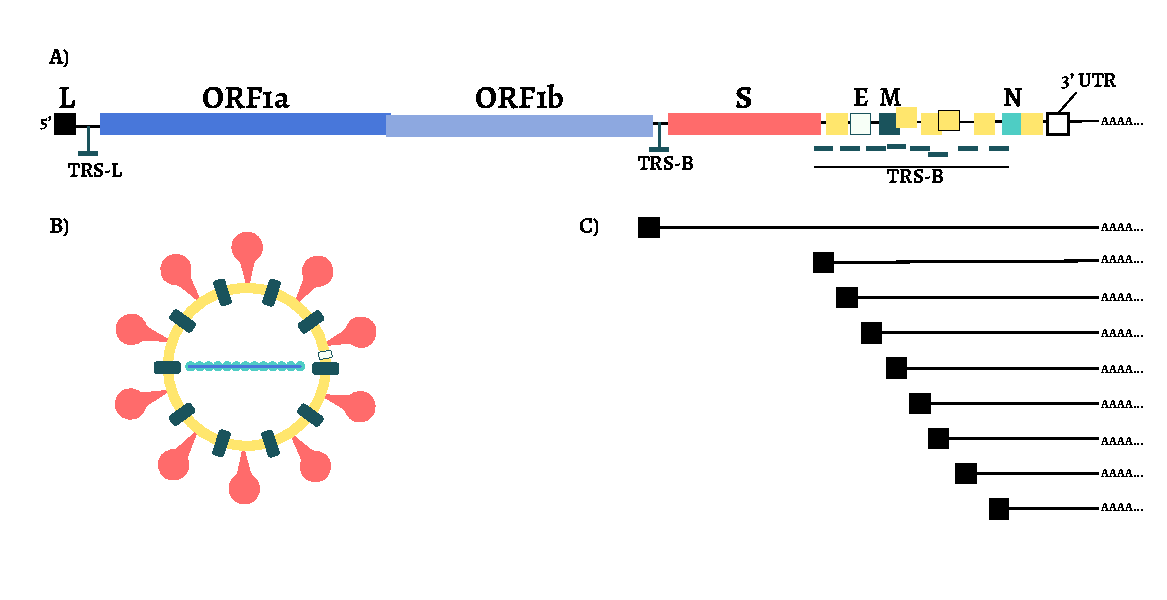
\includegraphics[width=\textwidth]{Figuras/Figura1}
 	\caption{A. Organización genómica del SARS-CoV-2. Los tamaños y distancias no son proporcionales a la realidad, es un esquema indicativo para facilitar la compresión. B. Estructura del virión. C.Transcritos generados por el proceso de síntesis discontinua}
 	\label{genoma}
 	
 \end{figure}
Entre los genes que codifican proteínas estructurales (S, E, M, N) se encuentran otros 7 ORF (señalados en amarillo en la figura \ref{genoma}) que codifican para proteínas accesorias.
 Debido a que en el presente trabajo se va a centrar más adelante en el RTC se ve conveniente deternese un poco en el proceso de replicación y transcripción del genoma. Dentro la síntesis de RNA RNA-dependiente de los coronavirus se diferencian dos procesos: la replicación (generando múltiples copias del genoma) y la transcripción de una colección de sgRNA (subgenómicos) que codifican para proteínas estructurales y accesorias. \\
 La replicación consiste en hacer copias enteras en menos (-) en forma de intermediarios replicativos que van a usarse como molde para generar el genoma en sentido positivo (+). Sin embargo, la transcripción es lo más característico de los \textit{Nidoviridae}, suponiendo un proceso de síntesis discontinuo para formar estos sgRNA, donde los TRS-B y -L juegan un papel fundamental.\cite{Kim2020}\\
 
 Los sgRNA tiene los mismos extremos 3' y 5' que el RNA genómico lo que implica que los sgRNA se sintetizan a partir de la fusión de secuencias no contiguas. Además, todos tiene en el extremo 5' la secuencia líder por lo que esta fusión se realiza a través de  la unión entre las secuencias L y B gracias a las características de los TRSs. Estos están formados por un núcleo conservado (CS, igual en todos los TRS) de unos 6-7pb con extremos variables.\\
 
 Comienza la síntesis de la hebra negativa, hasta que la RdRp se encuentra con una TRS y detiene la síntesis. En este punto se ha formado la cadena complementaria a CS (cCS-B) que se va a unir a la CS-L de la hebra positiva. Esto implica que se produzca un cambio del molde, se sintetiza la zona líder y se termina  como se puede observar en la figura \ref{repli}.
   
 Para la síntesis de RNA se realiza una transcripción discontinua, que produce un conjunto anidado en 3' y 5' RNA co-terminales subgenómicos (sgRNA). Durante la síntesis del RNA en sentido negativo el RTC y, en concreto la RdRp, al encontrarse con un TRS-B (formadas por un núcleo conservado de unas 6-7pb, CS, rodeado de secuencias variables) detiene la transcripción. Entonces se produce la unión entre TRS-B de la hebra negativa y la TRS-L de la positiva por complementariedad. \cite{nested}
 
  \begin{figure}[h]
 	\centering
 	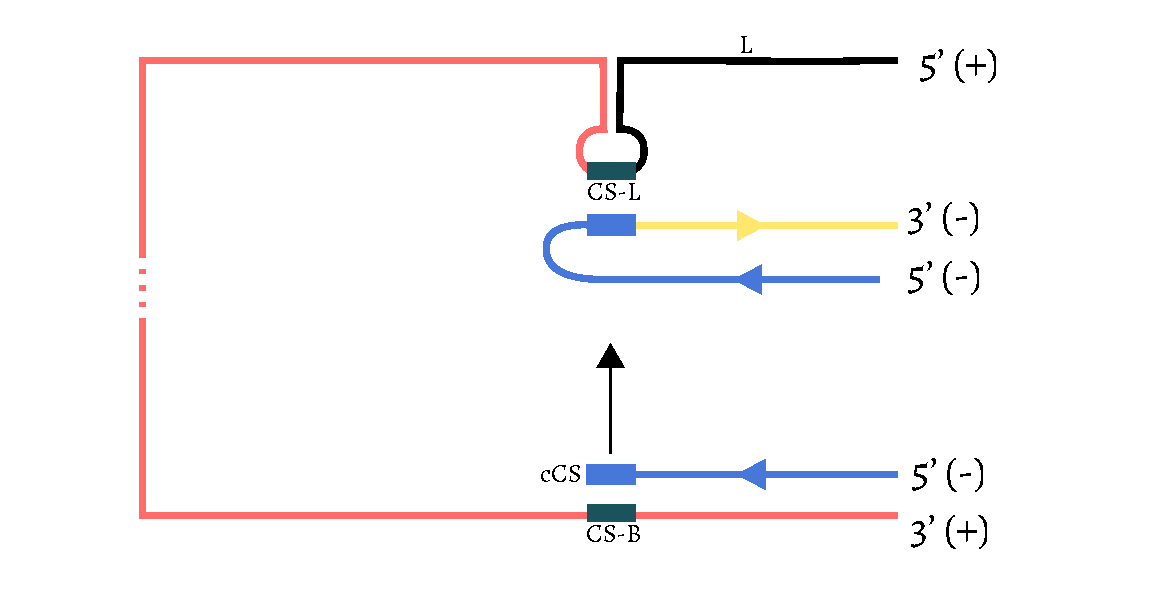
\includegraphics[width=\textwidth]{Figuras/Figura2}
 	\caption{Transcripción discontinua. La replicasa comienza a sintetizar la hebra negativa hasta que llega a un TRS-B, donde se detiene. Gracias a la complementariedad existente entre el cCS-B y el CS-L, la hebra menos se desplaza hasta el extremo 5' + terminando la síntesis con el fragmento complementario a la secuencia líder (amarillo)}
 	\label{repli}	
 \end{figure}
 

 \subsection{Ciclo viral: proteínas implicadas y aspectos funcionales}
 Quizás una de las proteínas más famosas del SARS-CoV-2 es la S o Spike debido a su papel en la vacunas que han salido al mercado, enfocadas a generar anticuerpos anti-S. Esto es debido a que S es la llave de entrada del virus, es la que permite que se produzca el primer paso de la multiplicación viral, la entrada en la célula. Es por ello que conviene detenerse un poco en la misma. Es una glucoproteína, siendo función unirse al receptor celular y mediar la entrada.
  Está formada por dos subunidades:
  \begin{itemize}
  	\item S1. Dividida a su vez en dos dominios funcionales N-terminal y C-terminal. Media la unión al receptor celular.
  	\item S2. Dominio transmembrana encargado de mediar la fusión de membranas.	
  \end{itemize}
En el extremo carboxiterminal de S1 tenemos la región RBD (receptor binding domain), que se va a unir al receptor celular ACE2 (angiotensina-Converting Enzyme 2). Al igual que otros coronavirus, el SARS-CoV-2 necesita un procesamiento proteolítico de la proteína S para activar la ruta endocítica e introducirse en el interior celular. Aquí es donde intervienen algunas proteasas celulares como TMPRSS2, cathepsina L y la furina. TMPRSS2 está altamente expresado junto con ACE2 en el epitelio nasal, bronquios y pulmones, lo que explica el tropismo tisular viral.\cite{natu}\\

 El dominio RBD tiene dos conformaciones principales, la acostada y la erguida. Mediante estudios de criomicroscopía electrónica se ha conseguido demostrar que en el SARS-CoV-2  está más tiempo en la forma acostada que en la erguida. Este es un detalle muy importante ya que permite al virus esconderse del sistema inmune y evadirlo de forma más eficaz al esconder el dominio de interacción, dificultándole el trabajo a los anticuerpos neutralizantes. \\

  Una vez se produce la fusión de membranas pasa al interior la nucleocápsida y comienza la expresión viral, altamente compleja tanto en el espacio y tiempo.
 \\El material génico viral se asemeja mucho a un ARNm eucariota, por lo que comienza directamente la traducción del ORF1a y ORF1b, produciendo dos grandes poliproteínas (pp1a y pp1ab, respectivamente). La eficiencia del cambio  de marco de lectura entre el ORF1a y b varía entre el 45-70\%, por lo que pp1 va a estar expresada entre 1.4-2.2 veces más que pp1ab.\\
 A partir de estas dos poliproteínas se van a generar 16 proteínas no estructurales:
 \begin{itemize}
 	\item pp1a:  nsp 1-11.
 	\item pp1ab: nsp 1-10, 12-16.
 \end{itemize}

El prosamiento de las poliproteínas se hace tanto de manera co-traduccional como post-traduccional a través de cortes proteolícos por dos cisteín proteasas en una noza localizada entre los genes de nsp3 y 5. nsp 5 se conoce como 3C-like proteasa o como proteasa principal (Mpro) debido a que es la responsable de la mayoría de los procesamientos. 

La nsp1 es liberada rápidamente para hacerse con el control de la maquinaria traduccional celular y permitir así la expresión del resto de genes. Las nsp2-11 forman el RTC viral. Van a determinadas localizaciones subcelulares y se cree que generarn las funciones necesarias para la acomodación del RTC (modulación de la membranas celulares, evasión inmune, proveer cofactores...). \cite{ciclo}\\\\

Las partes constituyentes del RTC y su funcionamiento será desarrollado en más profundidad en su apartado correspondiente. Dentro de sus funciones encontramos:

\begin{itemize}
	\item Síntesis de RNA. La realiza la RdRp (nsp12) junto con sus dos cofactores (nsp7 y 8). una función interesante es que nsp8 tiene actividad 3'-terminal-adeniltransferasa (primarasa)
	\item Corrección de errores. la realiza nsp14 y su actividad 3'-5' exonucleasa 
	\item Capping machinery. No está clara aún pero se sabe nsp14 tiene actividad N7-metiltransferasa y nsp16 tiene actividad O-metiltransferasa. Parece que nsp 13 y 10 también juegan un papel en el proceso
\end{itemize}

Una vez se han sintetizado todos los componentes se produce el ensamblaje de los mismos para así generar nuevos viriones que saldrán de la célula envueltos y listos para infectar a otras.
  
 \subsection{Respuesta inmunitaria y patología}
 
 Los coronavirus tienen maneras para evadir la respuesta inmune innata de diferentes maneras. Alguno de los mecanismos de escape consiste en esconder los PAMPs virales o los intermediarios replicativos (dsRNA) que activarían los receptores citosólicos. Por ejemplo, el dsRNA sería escondido por los DMVs (vesículas de doble membrana perinucleares). Muchas nsp que forman parte del RTC realizan funciones de evasión.
 Además, el virus posee mecanismos que retardan la secreción de interferón, lo que más tarde llevará a una respuesta inmune descontrolada e inmunopatologías. El hecho de que en los pasos iniciales de la infección por SARS-CoV-2 (causante de la COVID-19) hace que en un determinado punto se de una liberación excesiva de citoquinas pro-inflamatorias con infiltración celular en los pulmones causando daño en los tejidos. Los daños tisulares provocan una fibrosis (sustitución del tejido funcional del tejido por mecanismos de cicatrización) y se pueden dar infecciones bacterianas secundarias provocando neumonías. La descompensación de la respuesta inmnune puede ser tal que se da el síndrome de la tormenta de citoquinas

 
 \section{Posibles estrategias terapéuticas: Remdesivir}
 Existen diferentes puntos del ciclo de multiplicación viral donde podemos intervenir para formular compuestos anti-virales o para tratar de mejorar la respuesta inmune generada 
 
 \begin{itemize}
 	\item Inhibición de la entrada
 	\item Inhibición de la replicación viral (enfocándose en el RTC)
 	\item Agentes inmunomoduladores
 \end{itemize}

 Debido a que la estabilización del RTC es un proceso crucial en la replicación del virus, constituye un objetivo relevante a la hora de formular antivirales. Uno de los posibles objetivos podría ser Mpro, ya que es la proteasa encargada de la mayoría de procesamientos.\\ 
 Hay varios medicamentos disponibles que inhiben la replicación viral, entre los cuales encontramos remdesivir, favilavir, ribavirin, lopinavir y ritonavir. Excepto los dos últimos, todos los demás atacan a la RdRp. Estudios clínicos con el Remdesivir demostraron que los niveles de oxígeno necesarios para pacientes con la COVID-19 eran mucho menores en los pacientes tratados y ha demostrado actividad antiviral tanto \textit{in vitro} como \textit{in vivo}.
  
 Aquí van algunos datos del reporte final del Remdesivir \cite{remde}. En ensayos clínicos se vio que la media de tiempo de recuperación en pacientes con COVID-19 se vía reducida a 10 días, 5 menos que el grupo placebo. Además los que recibían el fármaco tenían una probabilidad mayor de recuperación al día 15. La mortalidad se reducía del 11.9\% al 6.7\%. Por tanto, se ve que el fármaco funciona pero, ¿cómo lo hace?.
 
 \begin{figure}[h]
 	\centering
 	\begin{subfigure}{0.75\textwidth}
 		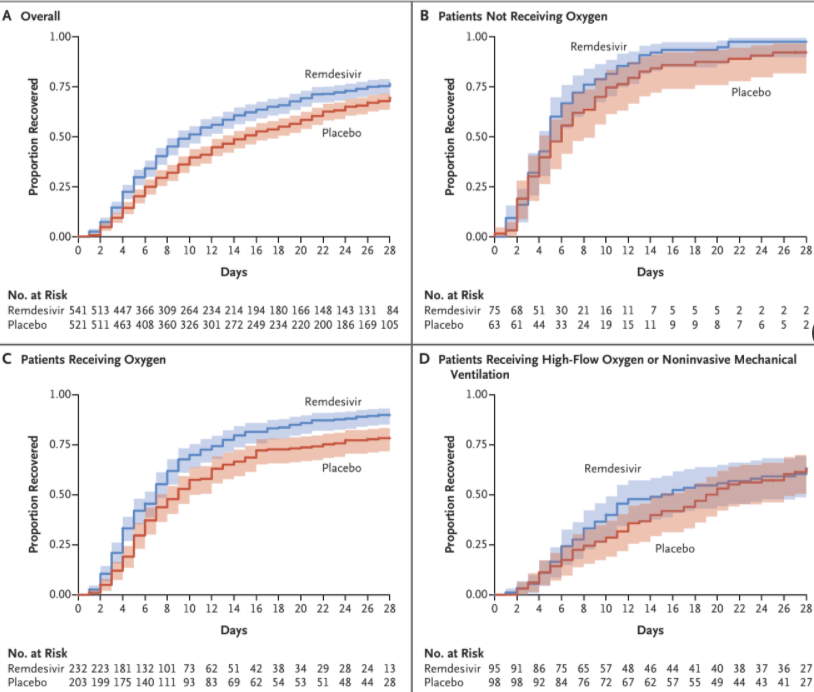
\includegraphics[width=\linewidth]{Figuras/Figura10}
 		\caption{Gráficos del estudio clínico de Remdesivir \cite{remde} }
 	\end{subfigure}   
    \begin{subfigure}{0.35\textwidth}
    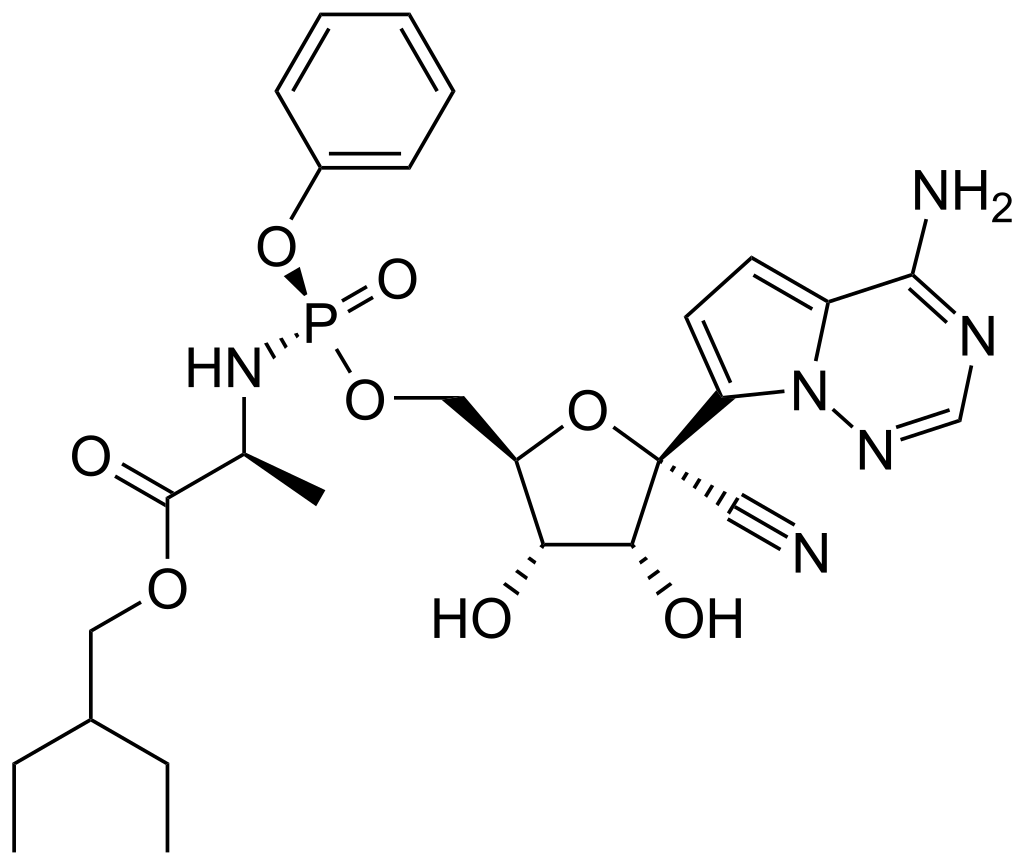
\includegraphics[width=\linewidth]{Figuras/Figura11}
    \caption{Estructura química del Remdesivir}
    \label{fig: remde}
    \end{subfigure}
 	
 	
 \end{figure}
 
 Bueno pues el Remdesivir (o GS-5734) es un inhibidor de la polimerasa viral (RdRp) con actividad inhibitoria contra el SARS-CoV-1 y el MERS-CoV. Por ello, se propuso su uso en el SARS-CoV-2. Es inhibidor de la transcripción de manera no obligada y, en terminología farmacéutica es utilizado como profármaco. Esto quiere decir que se administra en forma y va a sufrir una serie de transformaciones hasta que alcanza su forma activa. Se administra como monofosforamidato y cuanto entra a la célula pasa a Remdesivir Monofosfato (RMP), pero para que pueda actuar se necesita que pase a su forma activa, Remdesivir Trifosfato (RTP). El Remdesivir es, por tanto, un profármaco monofosforamidato de un análogo de adenosina que va a ejercer una inhibición competitiva de RdRp.
 Su estructura química se puede ver en la figura \ref{fig: remde}.  \\
  RTP tiene una estructura similar al ATP por lo que van a competir por la unión a la RdRp \cite{remde2}. Cuando RTP entra en la síntesis se va a unir a la posición i de la cadena de RNA en síntesis, lo que lelva a la terminación en la posición i+5 de manera general. Así se termina la replicación viral.
  
  Según datos expermientales de \cite{estremde} la extensión del RNA primer siempre se termina cuando hay una alta concentración de RTP y el ratio RTP/ATP es bajo. Además, según estructuras se puede observar que el RMP  se une de manera covalente al extremo 3' de la hebra primer, en concreto al residuo +1. A pesar de que haya un exceso de RTP siempre va a haber una RMP en la hebra primer.
  
  \begin{figure}
  	\centering
    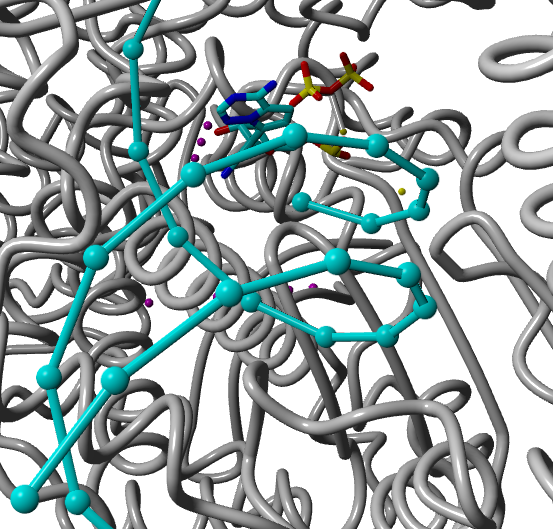
\includegraphics[width=0.4\linewidth]{Figuras/Figura37}
  	\caption{Gris: nsp12, Cian: RNA. Se ve como el Remdesivir interactúa tanto con el RNA como con nsp12, logrando parar la replicación del genoma}
  \end{figure}
  
 
 RMP se posiciona en el centro del sitio activo y como un análogo de la adenosina monofosfato, crea interacciones con una base de la hebra primer y dos enlaces de hidrógeno con una uridina de la molde. Además interacciona con las cadenas laterales de K545 y R555. También interacciona con las iones magnesio y el pirofosfato, esenciales para la actividad. El pirofosfato es la puerte del canal de entrada nucleotídica, bloqueando la entrada de NTP. \cite{estremde}
 
 Algunos conceptos serán desarrollados en el siguiente punto, donde se explicará el RTC en mayor profundidad.

 
 \section{Complejo Replicación Transcripción}
 La mayoría de las nsp codificadas por el gen de la replicasa, junto con la proteína N y un número desconocido de proteínas celulares se asocian en un RTC asociado a la membrana viral que media tanto la replicación como la síntesis de los sgRNAs. Dentro de este gran complejo las proteínas esenciales son la RdRp (nsp12), la helicasa (nsp13) y el complejo nsp7-nsp8 (cofactores de nsp12), los cuales se pueden ver en la figura \ref{todos}. Debido a su especial importancia, se van a desarrollar en mayor profundidad.
 
 \begin{figure} [h]
 	\centering
 	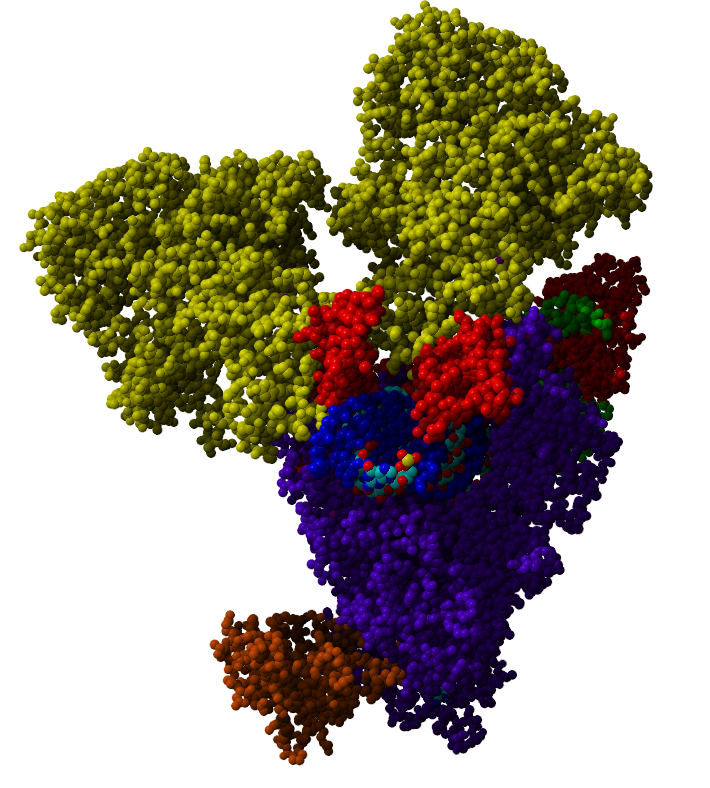
\includegraphics[width=0.4\linewidth]{Figuras/Figura38}
 	\caption{Estructura del ERTC. Morado: nsp12. Amarillo: 2 nsp13. Rojo: 2 nsp8. Verde: nsp7. Naranja: nsp9. Azul: Template RNA. Cian: Primer RNA}
 	\label{todos}	
 \end{figure}

  \begin{figure}[h]
 	\centering
	 \begin{subfigure}{0.3\textwidth}
	 	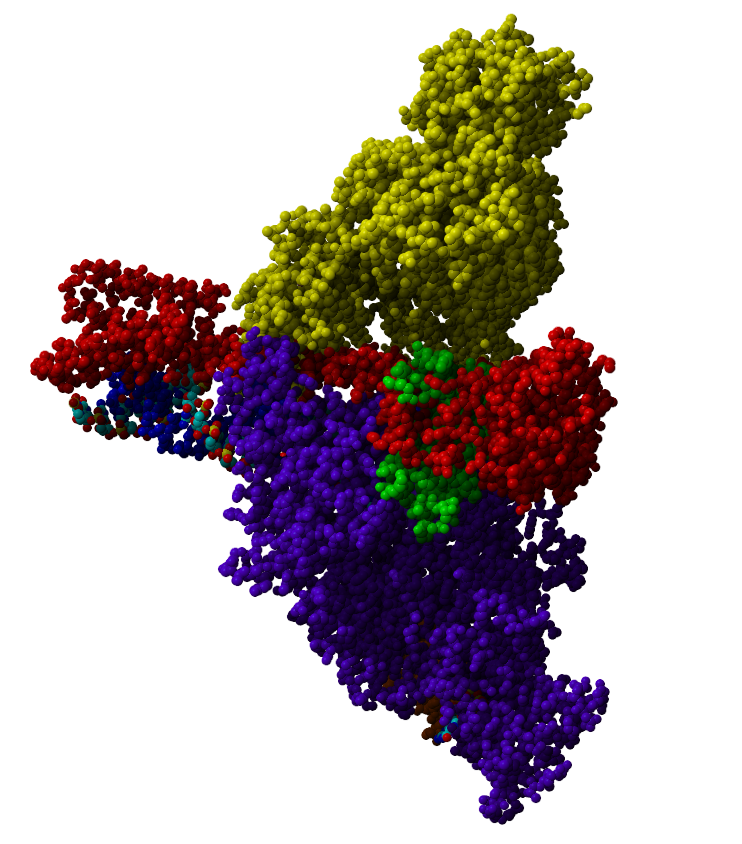
\includegraphics[width=\linewidth]{Figuras/Figura39}
	 	\caption{Derecha} 	
	 \end{subfigure}
	 \begin{subfigure}{0.3\textwidth}
	 	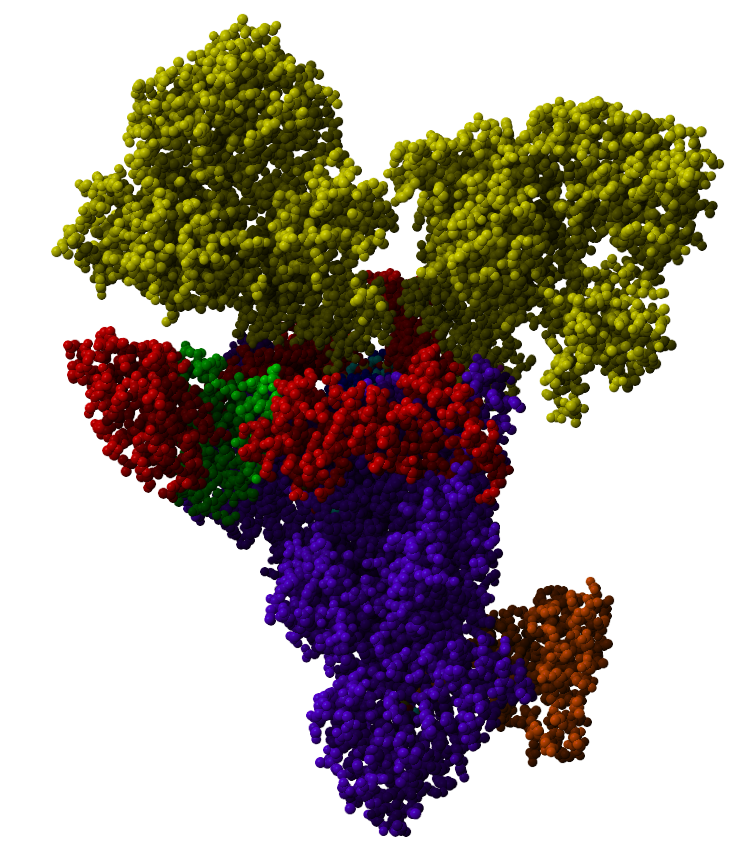
\includegraphics[width=\linewidth]{Figuras/Figura40}
	 	\caption{Atrás} 	
    \end{subfigure}
	 \begin{subfigure}{0.3\textwidth}
		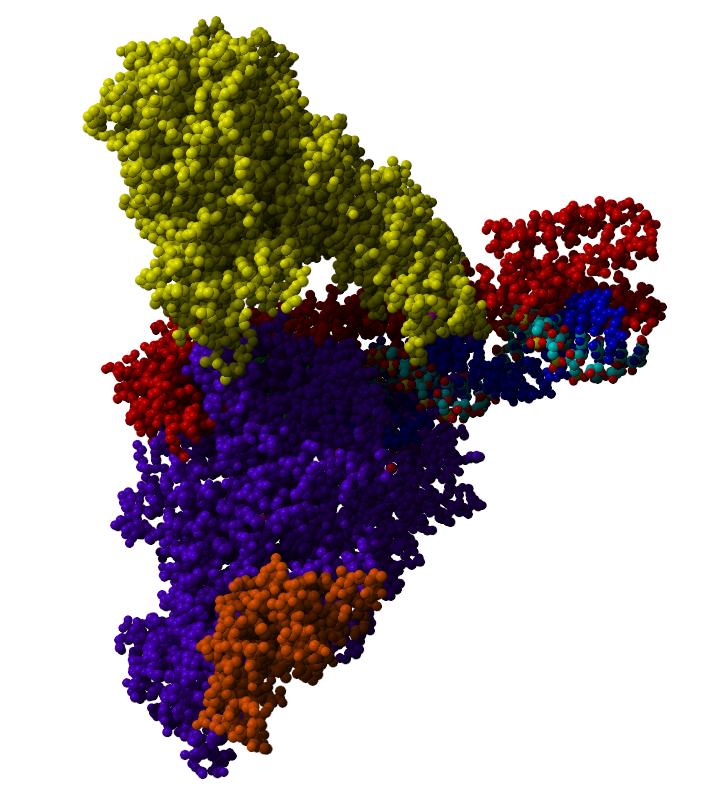
\includegraphics[width=\linewidth]{Figuras/Figura41}
		\caption{Atrás} 	
	\end{subfigure}
  \caption{Estructura del ERTC. Morado: nsp12. Amarillo: 2 nsp13. Rojo: 2 nsp8. Verde: nsp7. Naranja: nsp9. Azul: Template RNA. Cian: Primer RNA}
  
 \end{figure}
 
 \subsection{RdRp (nsp12)}
 En la estructura de la nsp12 del SARS-CoV-2 diferenciamos los siguientes dominios:
 \begin{itemize}
 	\item Dominio polimerasa, RdRp (residuos 366-932). Su estructura recuerda a una mano derecha y se divide en
 	\begin{itemize}
 		\item Dedos (366-581, 621-679)
 		\item Palma (582-620, 680-815)
 		\item Pulgar(816-932)
 	\end{itemize} 
 	\item Dominio NiRAN (4-249). Extensión N-terminal específica de los nidovirus que adopta la arquitectura de nucleotidiltransferasa asociada a RdRp.
 	\item Dominio Interface (250-365). Une a RdRp con NiRAN.
 \end{itemize} 
Dentro de NiRAN, en concreto en la región 29-50 (marcada en rojo en la figura \ref{1º}), se encuentra un dominio de horquilla $\beta$ que se inserta la ranura formada por NiRAN y el subdominio de la palma del dominio RdRp. Esta horquilla-$\beta$ crea una serie de contactos cercanos entre estos dominios estabilizando la estructuta general\\

La RdRp del SARS-CoV-2 tiene una serie de aspectos claves diferenciadores de la de su hermano el SARS-CoV. En los residuos desde N215 hasta D218 se forma una lámina $\beta$, estando los residuos de forma más ordenada que en la SARS-CoV nsp12. Esta región contacta con la hebra formada por los residuos del V96 al A100, contribuyendo a la estabilización de la conformación. Como resultado se forma un compacto semibarril-$\beta$. \\
En las estructuras realizadas en ausencia de DTT se observó la formación de enlaces disulfuro entre los residuos C301-C306 y C487-C645, mientras que cuando hay DTT se observan iones de zinc. Estos iones de zinc están muy conservados teniendo una función importante en la estabilización de la estructura.

 \begin{figure}
	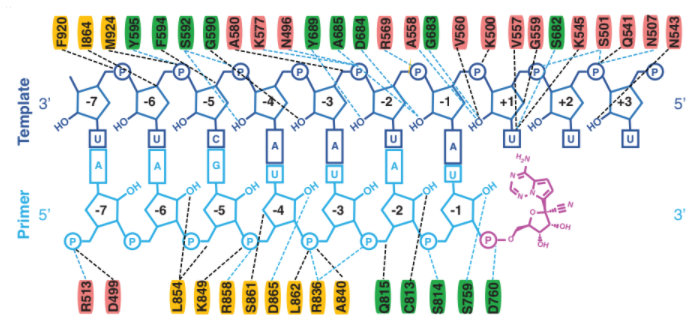
\includegraphics[width=\linewidth]{Figuras/Figura45}
	\caption{Contacto de nsp12 con el esqueleto de ribosa. También se puede apreciar la unión del Remdesivir a la hebra primer (Zhang \& Zhou, 2020)}
	\label{fig: contremde}
\end{figure}

El sitio activo del domino RdRp está formado por los motivos conservados A-G de la polimerasa, cuya organización se puede ver en la figura \ref{1º}. El \textbf{motivo A} va desde el residuo 611 al 626 y tiene el residuo de unión a cationes divalentes clásico que está conservado en la mayoría de polimerasas virales (D618). Otro motivo muy conservado es el C (753-767), situado en la horquilla entre dos hebras $\beta$.  El hecho de que estén tan conservados indican que son esenciales para su función. 
En esta estructura, tal y como ocurre en otras polimerasas, los canales de entrada de NTP, del molde y el de salida de la hebra naciente están positivamente cargados y son accesibles para el disolvente. Además, todos convergen en la cavidad central donde los motivos median la síntesis de RNA a partir del molde.
El canal de entrada de NTP está formado por un set de seriduos hidrofílicos del motivo F (K545, R553 y R555). El RNA molde entra al sitio activo de los motivos A y C a través del surco formado por los motivos F y G. El motivo R y el subdominio del pulgar apoyan al primer. El híbrido molde-producto sale del sitio activo por el tunel de salida al frente de la polimerasa. \cite{RdRp}

  \begin{figure}[h!]
 	\centering
 	\begin{subfigure}[h]{0.45\textwidth}
 		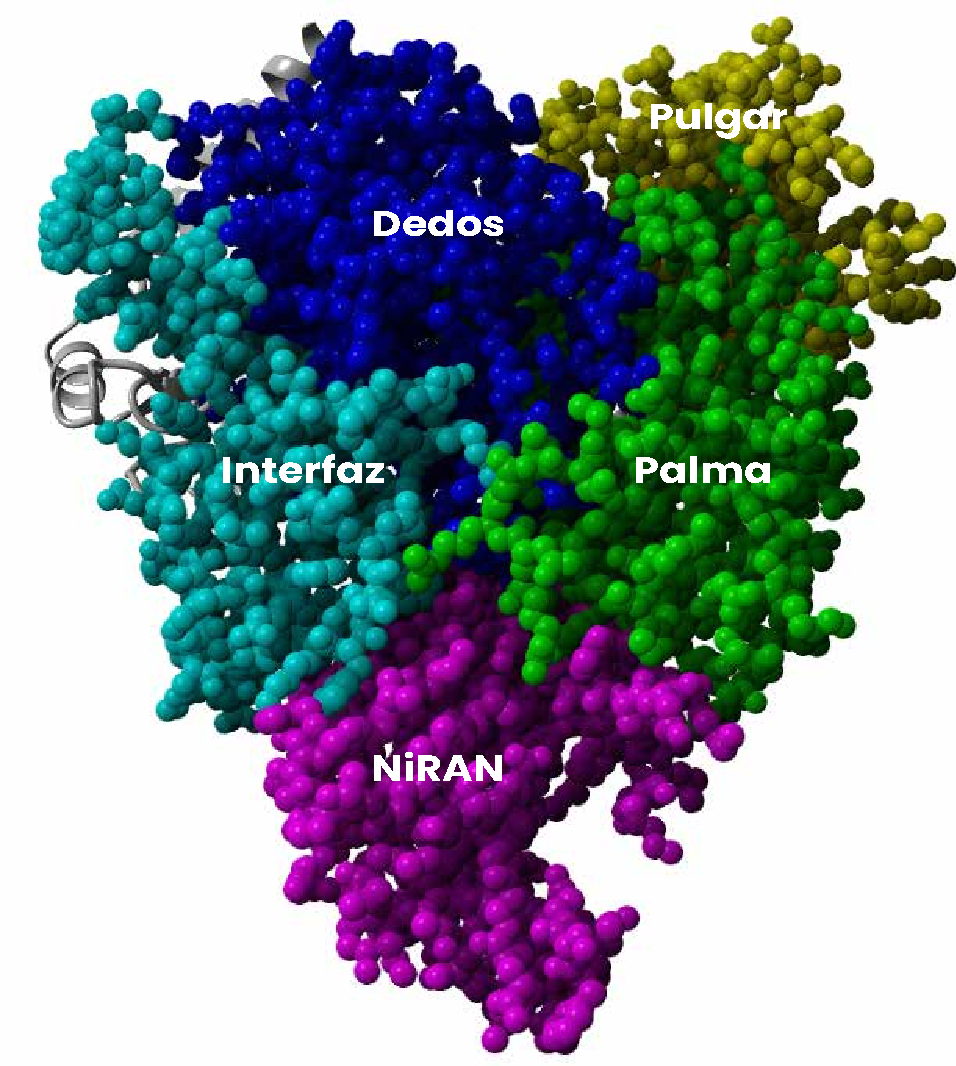
\includegraphics[width=\linewidth]{Figuras/Figura4}
 		\caption{}
 		
 	\end{subfigure}
 \begin{subfigure}[h]{0.45\textwidth}
 	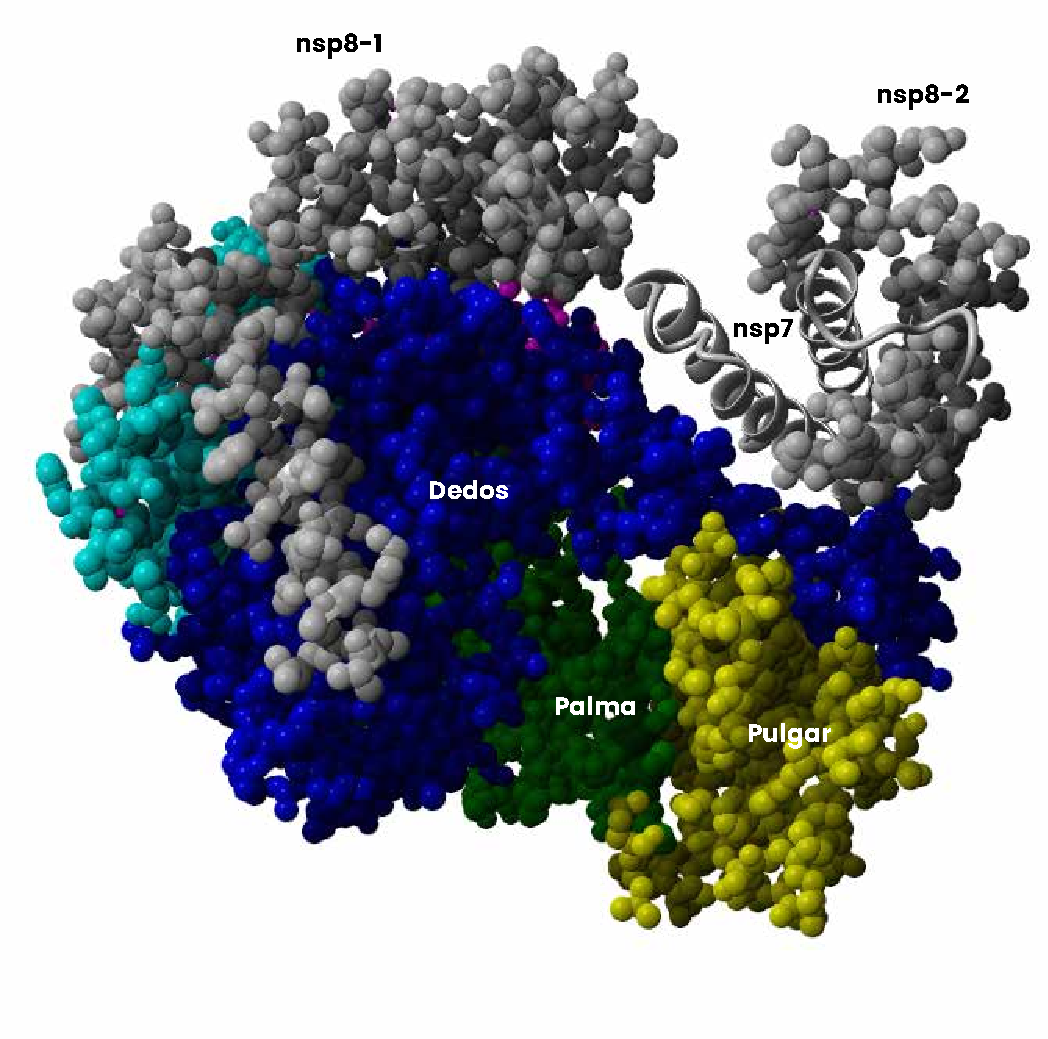
\includegraphics[width=1.2\linewidth]{Figuras/Figura6}
 	\caption{ }
 	
 \end{subfigure}
\begin{subfigure}[h]{0.45\textwidth}
	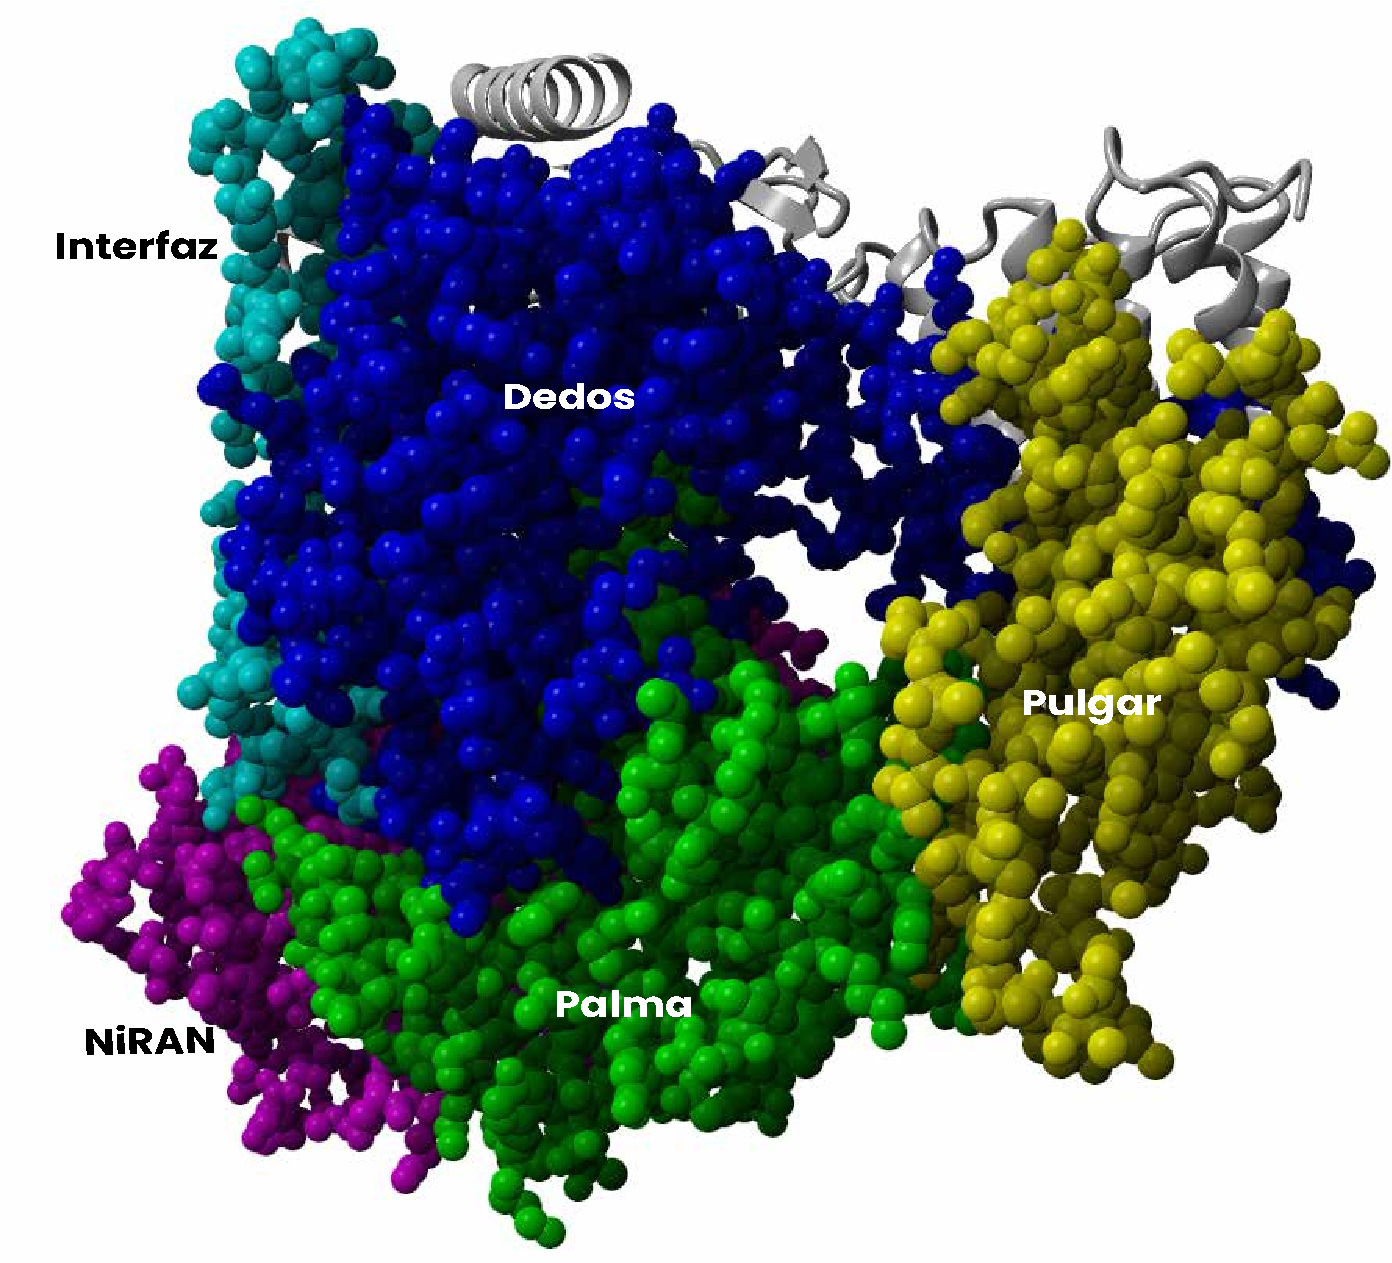
\includegraphics[width=\linewidth]{Figuras/Figura5}
	\caption{}	
\end{subfigure}
\quad
\begin{subfigure}[h]{0.35\textwidth}
	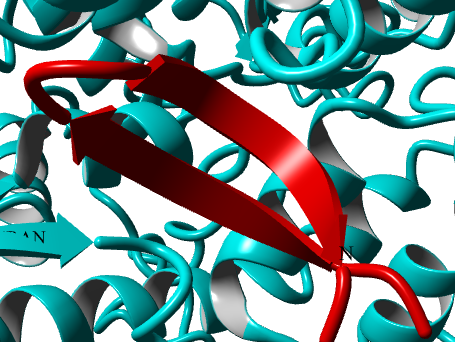
\includegraphics[width=\linewidth]{Figuras/Figura44}
	\caption{Horquilla $\beta$ específica de SARS-CoV-2}
	\label{1º}	
\end{subfigure}
\quad

\begin{subfigure}[h]{\textwidth}
	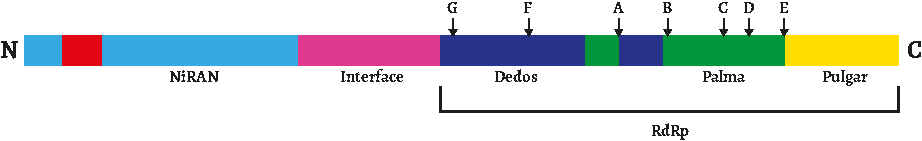
\includegraphics[width=\linewidth]{Figuras/Figura7}
	\caption{}
	\label{1º}	
\end{subfigure}



 \label{nsp12}
 \caption{Imágenes desde diferentes puntos de vista en (a), (b) y (c) de nsp12 en asociación con nsp8 y 7. (d) Representación de la estructura primaria de la proteína}
 \end{figure}

En el centro activo se pueden ver también dos iones magnesio y un pirofosfato. 
\subsection{nsp7-nsp8}
El complejo nsp7-nsp8 tiene una estructura conservada, similar a la del SARS-CoV. Los estudios estructurales en el SARS-COV indican que nsp8 forma estructuras hexadecaméricas junto con nsp7 generando un hueco en el que se puede depositar dsRNA, lo que sugiere que posee actividad primarasa. \cite{78}

Nsp7 tiene una longitud de 83 aminoácidos y su plegamiento consiste en cuatro hélices con diferente posición y orientación en función si está aislado o formando el supercomplejo con nsp8 lo que indica que está fuertemente afectada por la interacción (sobre todo la $\alpha$4). Además, gracias a estudios de reverso genética se confirmó su importancia en la replicación viral. \\

Nsp8 tiene un tamaño de unos 200 aminoácidos y en los inicios se dudaba entre dos estudios uno en el que formaba un a estructura hexadecamérica con 8 copias de nsp7-8 yuna segunda con una actividad RNA polimerasa específica de nsp8, que implicaba mecanismos de síntesis de RNA. Esta acticada se veía en presencia de cationes divalentes de manganeso o magnesio generando productos de máxiumos 6 nucleótidos. Nsp8 tiene dos dominios que recuerdan a un palo de golf (Figura \ref{fig: nsp8}): cabeza y extensión. \\

\begin{figure}[h!]
	\centering
	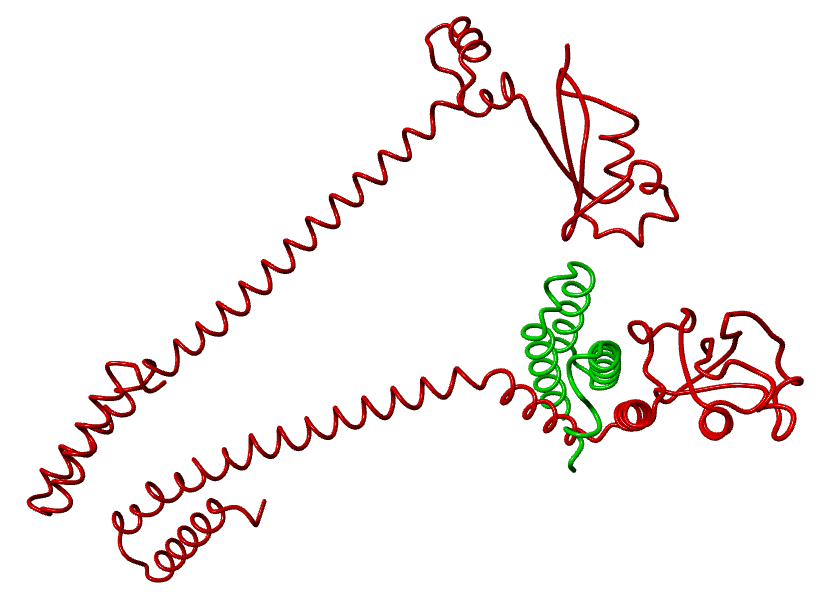
\includegraphics[width=0.8\linewidth]{Figuras/Figura43}
	\caption{Imagen de la estructura secundaria de nsp7 (verde) y dos nsp8 (rojo) dentro del complejo. Se puede observar la estructura de palo de golf de nsp8}	
	\label{fig: nsp8}
\end{figure}

El complejo hexadecamérico tiene forma de donut con un canal dentral con cadenas lateralas positivas.Se pensó que constituiría un complejo que deslizaría a lo largo del RNA en replicación junto con las otras proteínas, consituyendo un factor procesivo de RdRp.

A parte de este compejo hexadecamérico, nsp8 adopta dos conformaciones "palo de golf" y "palo de golf con el eje doblado". Estudios de reverso genética en en SARS-COV demostraron que los residuos P183 y R190 (interacción con nsp12) y el K58 (interacción con RNA) eran esenciales.  \cite{biblia}

Por todos estos datos se pensaba que el complejo ejercería un efecto de primasa. Sin embargo, en los estudios recientes del C-RTC sugieren que el dímero nsp7-8 está muy alejado del sitio activo de nsp12, por lo que no puede actuar como primasa, por lo menos en cis. El dímero nsp7-8 se superpone bien tanto en la estructura hexadecamérica como en la en el dímero unido a nsp12.

Está claro que el complejo juega un papel importante durante la replicación, pero se deben de realizar más estudios para determinar cuál es.

Este complejo está formado por una nsp12, una nsp7 y dos nsp8. Tiene una alta similaridad al del SARS-CoV con un RMSD de 0.82 para los C$\alpha$. \cite{miniRTC}

\subsection{nsp13}
Pertece a la superfamilia 1B (SF1B) y puede separar tanto DNA como RNA de manera NTP dependiente con polaridad 5'-3'. Además, a parte de la actividad helicasa también presenta una actividad RNA 5'-trifosfatasa lo que implica que podría jugar un papel importante en la maquinaria de capping.
\cite{helicasa}

Las helicasas SF1 tiene dos dominos RecA ATPasa canónicos (RecA1, 234-438, RecA2, 439-601), pero las helicasas de los nidovirus tienen tres dominios característicos: N-terminal dominio de unión a zinc (ZBD, 1-100), el tallo (100-149, 229,234), y el dominio 1B (Figura \ref{13}). Las funciones de cada dominio siguen sin estar claro, pero variaciones en los mismos suponen un descenso de la actividad helicasa y en la propagación viral. 

Se piensa que el ZBD es esencial, siendo capaz de modular la función de la helicasa debido a al importancia vista en la presencia o no de zinc.

Nsp13 interactúa con nsp12. En las estructuras consultadas se ven dos nsp13 unidas al RTC. nsp13-2 nunca se encuentra a no ser que nsp13.1 ya esté y es disociable, cosa que no ocurre con nsp13.1 que está fuertemente unido gracias a las interacciones entre el ZBD con el pulgar de nsp12 y nsp8. 

\begin{figure}[h!]
	\centering
	\begin{subfigure}[h]{0.45\textwidth}
		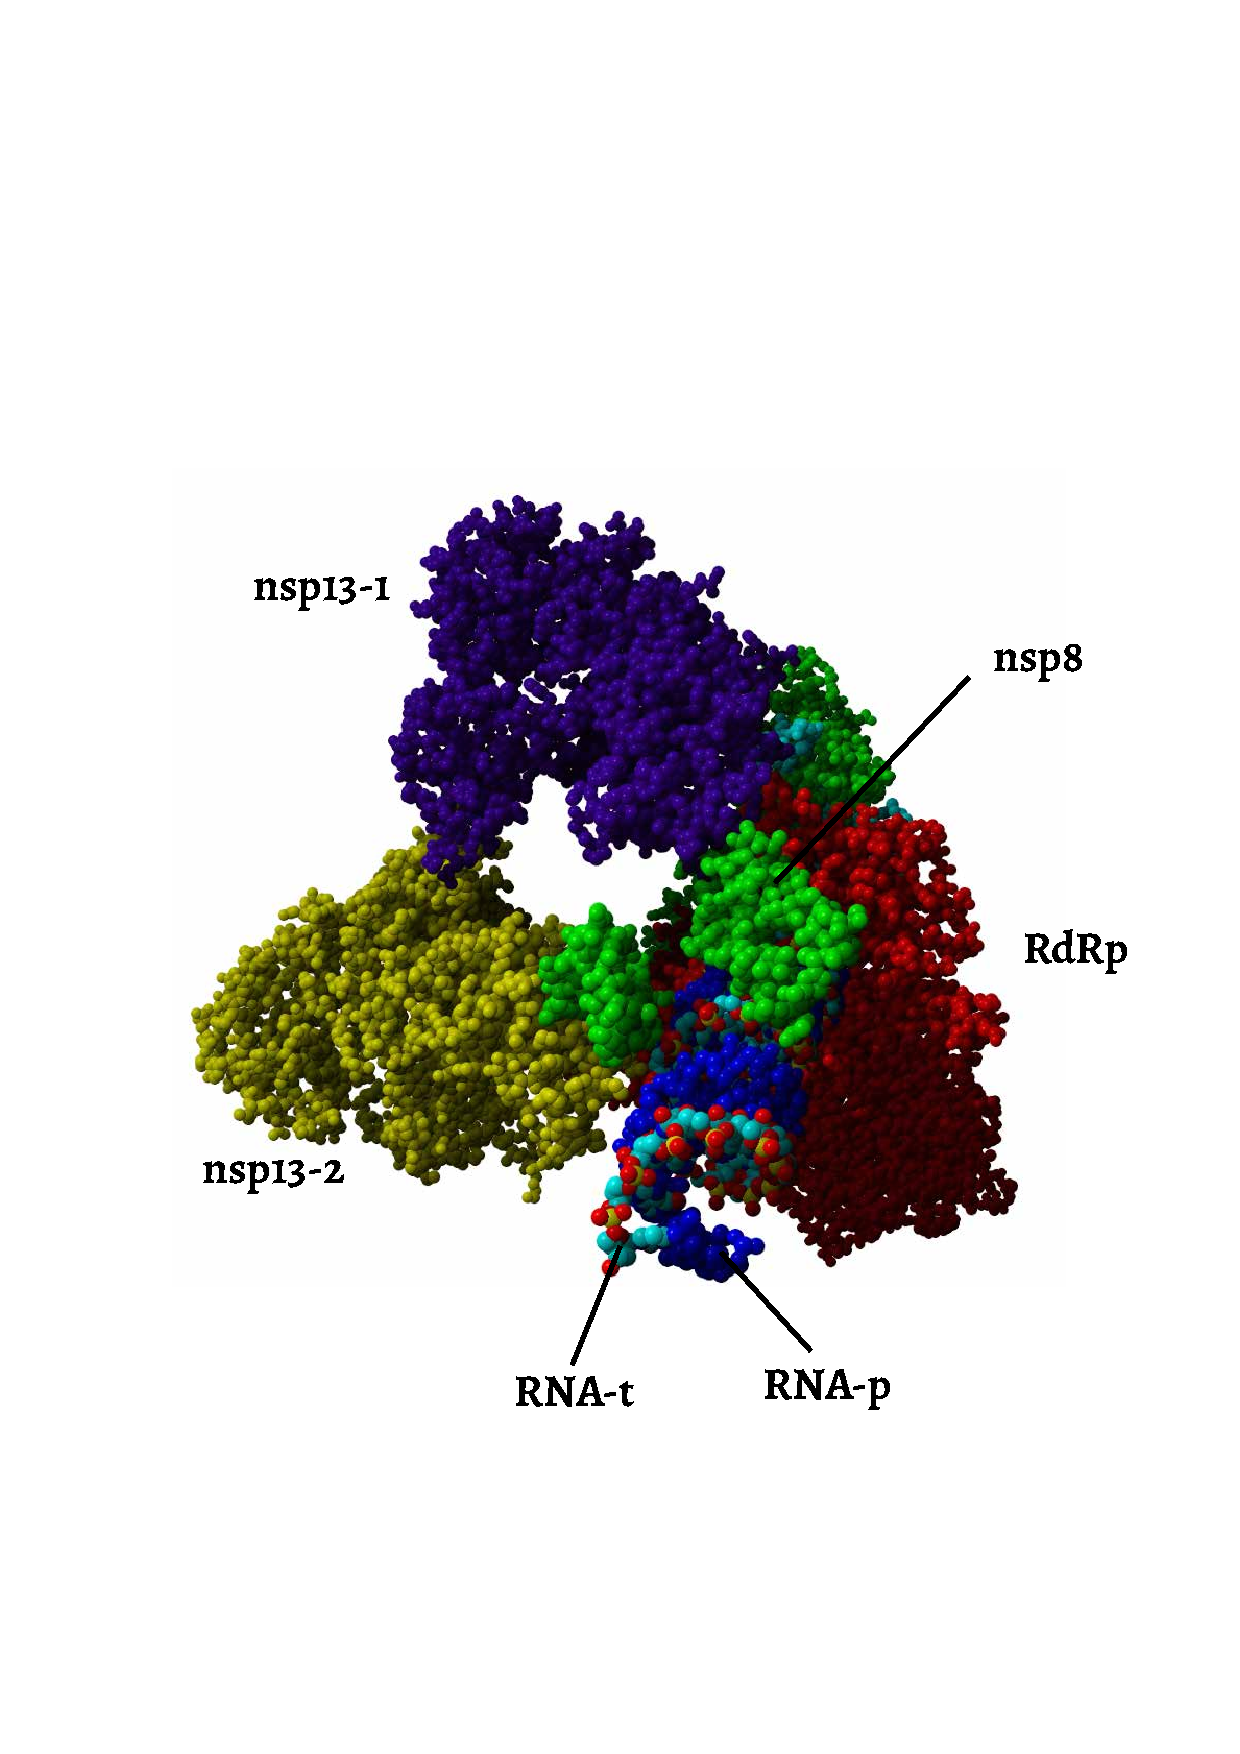
\includegraphics[width=1.2\linewidth]{Figuras/Figura8}
		\caption{Complejo nsp12-nsp8-nsp7-nsp13-RNA. RNA-t se correponde con el molde y RNA-p se corresponde con el producto generado}		
    \end{subfigure}
    \begin{subfigure}[h]{0.45\textwidth}
		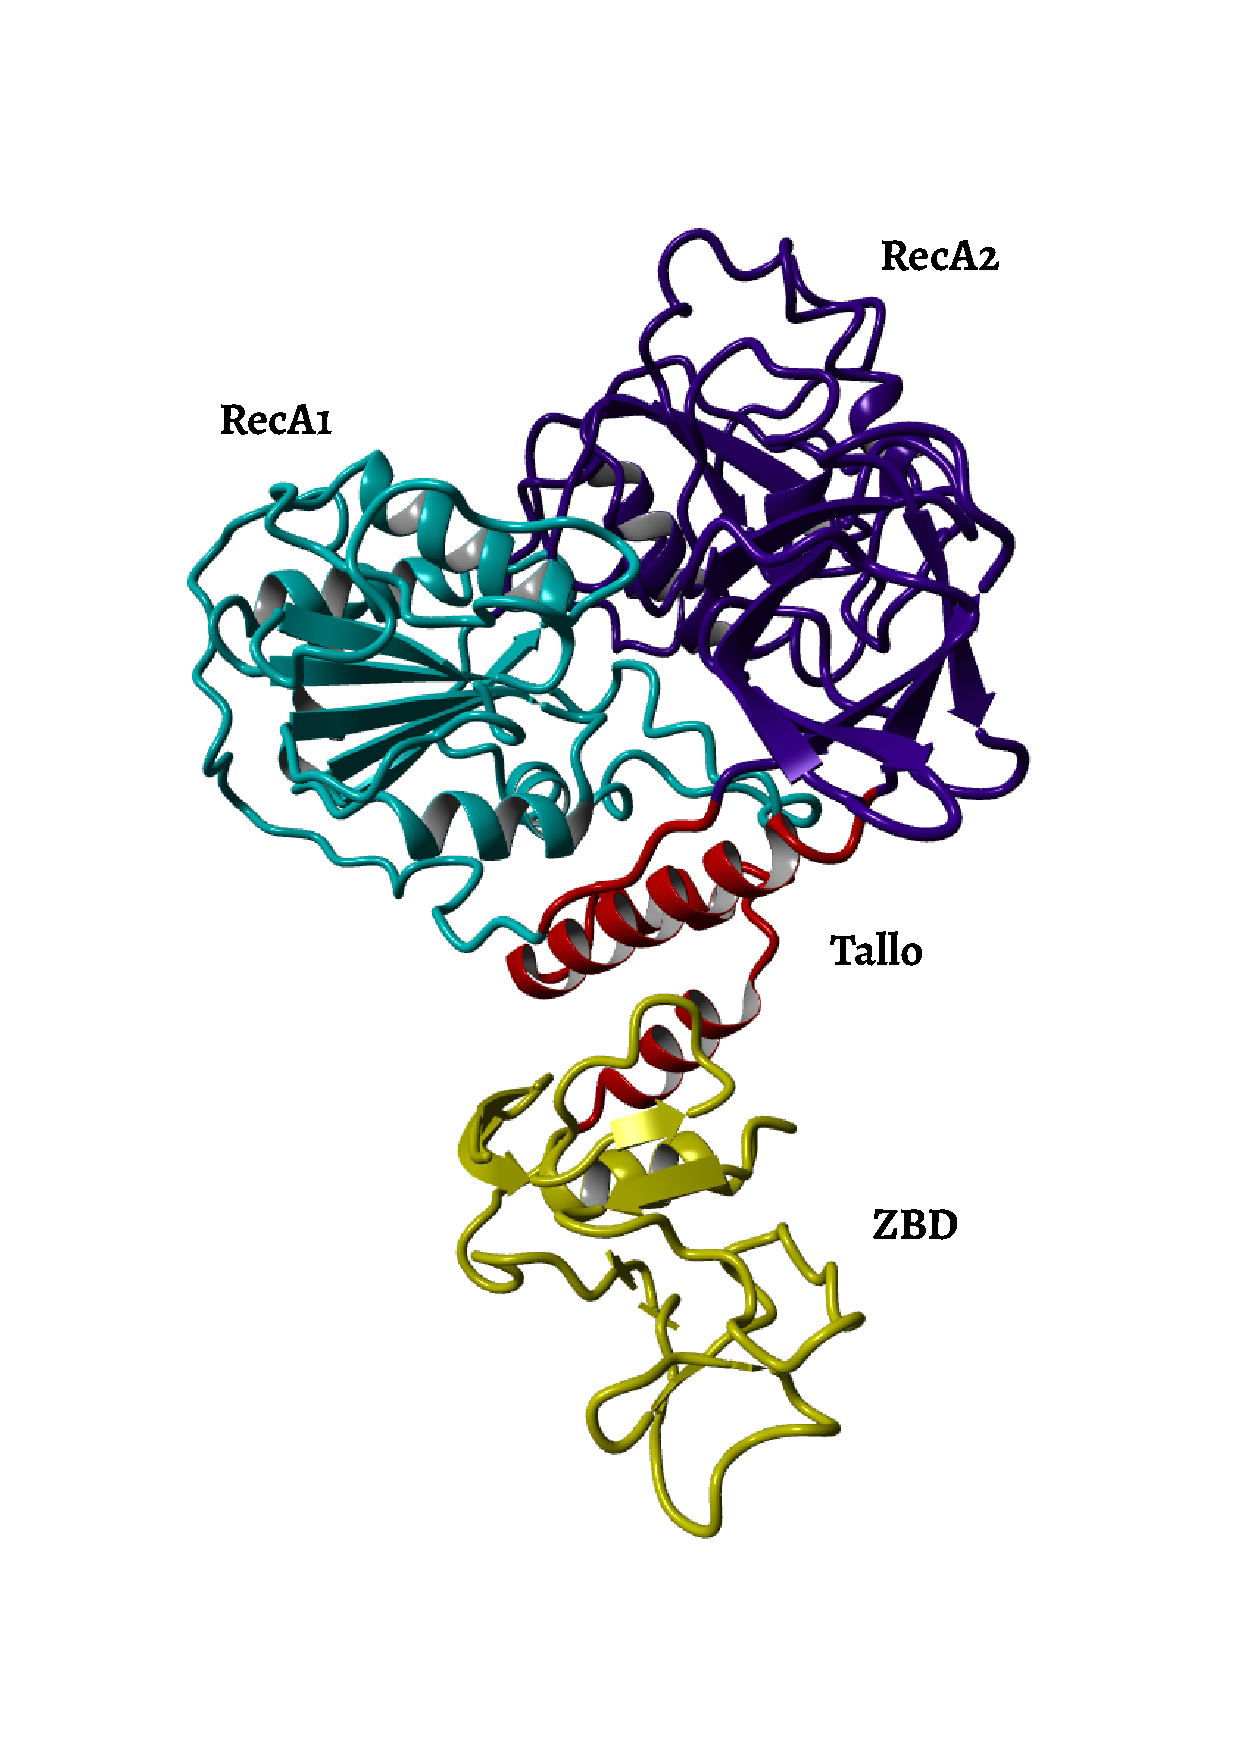
\includegraphics[width=1.2\linewidth]{Figuras/Figura9}
		\caption{Estructura nsp13}		
		\label{13}
	\end{subfigure}
   
   \caption{Imágenes del complejo miniRTC con las dos nsp13}
   
\end{figure}

\subsection{nsp9}
La proteína nsp9 tiene alrededor de 110 aminoácidos de longitud y es el segundo producto de corte del gen de la replicasa, después de nsp5. 
En estudios recientes se ha visto que nsp9 se une a nsp12 en un sitio cercano al centro activo de NiRAN. La interfaz nsp9-nsp12 tiene dos regiones definidas. La primera está formada por el extremo N-terminal de nsp9, el dominio de la palma y la horquilla $\beta$. Se produce una interacción por enlaces de hidrógeno entre los residuos D36, Y728 y R733 con el N2 de nsp9.
En la segunda región, la región plana de NiRAN interacciona con el extremo C-terminal de la $\alpha$ hélice de nsp9, estabilizado por gran cantidad de interacciones hidrofóbicas y tres enlaces de hidrógeno.

En el SARS-CoV se ha creído que la forma biológicamente activa es un dímero capaz de unir ácidos nucleicos con apetencia por el RNA de cadena simple. Esto podría deberse a que puede que nsp9 tenga una forma intermediaria donde forma un homodímero para después unirse de manera monomérica al RTC.
\cite{eRTC} 

\subsection{E-RTC}
El RTC extendido está formado por una nsp7, dos nsp8, una nsp12, 2 nsp13, emparejado con el RNA primer-molde y una nsp9. Estudios de microscopía.
La región pareada del RNA molde-primer está ligeramente sujetada por nsp12 y los dos palos helicales de nsp (IMAGEN). Dos protómeros de nsp13 se unen a la región plana formada por las dos nsp8 y nsp12. Nsp13-1 se une a nsp12 y a nsp8-1, estabilizando la arquitectura del RTC, mientras que el nsp13-2 guía al extremo 5' deshibridado del RNA molde a través del canal que forma con sus dominios 1A, 2A y 1B.

En la estructura obtenida por \cite{helicasa} el centro activo de NiRAN se ve una unión a ADP-Mg2+, con una interacción iónica entre la H75 con la adenina. Sin embargo, este no es un residuo conservado lo que nos lleva a pensar tres opciones. O bien no es una unión determiannte, que la especificidad de bases varía ente especies o que no tiene especificidad en su actividad. Se necesitan más estudios para estudiar la actividad enzimática de NiRAN.

En las DdRps celulares (DNA dependiente RNA polimerasa) hay un elemento estructural conservado que divide el sitio activo, un puente en hélice. Canal secundatio que permite que los NTP entren al sitio activo para unirse al extremo 3' creciente.

En la RdRp viral, la estructura que separar las hebras en el motivo F con su bucle en horquilla beta. El canal secundario de las RdRp está perfectamente posicionado para acomodar el RNA. Basados en esta analogía estructural \cite{helicasa} proponen que la RdRp viral debe de ir hacia a´tras y el extremo monocatenario del RNA en 3' debe de salir por el canal secundario.


El extremo N-terminal de nsp9 se inserta en el interior del centro catalítico de NiRAN y forman enlaces con GDP. Los residuos de contacto con GDP están muy conservado entre diferentes coronavirus. Las función biológica exacta de nsp9 no está del todo clara pero se piensa que tiene un papel importante en la regulación del capping junto con nsp14 (N7-Metilasa) y nsp16 (2'-O-Metilasa).

El RNA molde se sujeta por los subdominios dedos, palma y pulgar produciendose interacciones con un total de hasta 41 residuos de nsp12 y, aunque nsp7-8 son necesarias para que nsp12 una el RNA, no se ven interacciones entre estas y el RNA. La mayoría de interacciones entre la proteína y el RNA se realizan a través de los -OH en 2' del esqueleto de fosfato-ribosa. Esto es esencial ya que le permitiría al complejo distinguir entre RNA y DNA. No se producen interacciones entre nsp12 y las bases nucleotídicas, indicando que es una unión independiente de la secuencia.



\cite{eRTC} 



 \chapter{Actividades del CPA}
 \section{Bases de datos secuenciales y estructurales}
 \subsection{Detección de formatos de ficheros proteicos y extracción de la secuencia primaria}
 Desarrollar un diagrama de flujo que permita identificar si un fichero tiene formato EMBL, UniProt, GenBank, PDB u otros  diferentes. A continuación, desarrollar un programa informático capaz de discriminar automáticamente entre tres de ellos: Genbank y UniProt y PDB y muestre en pantalla las secuencias primarias de las proteínas correspondientes en códigos de una letra. Emplear ese programa con los ficheros bajados de Internet de la proteína asignada.
 
 En esta actividad se pedía crear una herramienta capaz de detectar el formato de un fichero y de extraer la secuencia primaria de la proteína del mismo. Para su realización se desarrolló un sistema de identificación de cada fichero basado en su formato, debido a que cada uno tiene características diferenciales.
 
El programa creado es capaz de diferenciar entre cuatro tipos distintos de fichero y es capaz de extraer la secuencia de tres de ellos. 
\begin{itemize}
	\item Ensemble. Su primeros dos caracteres son ID, y los primeros caracteres de la segunda fila son XX
	\item UniProt. Sus primeros dos caracteres son ID, y los primeros caracteres de la segunda fila son AC
	\item GenBank. Sus primeros caracteres son LOCUS
	\item PDB. Sus primeros caracteres son HEADER	
\end{itemize}

 \subsection{Desarrollo de la función CargarPDB}
 Algo esencial para la realización de todos los análisis proteicos es generar una herramienta que pueda extraer la información de un fichero (pdb en este caso) para sí poder realizar diferentes cálculos con ellos.
 
CargarPDB es una función muy potente que permite acceder rápidamente a la información que nos interese. Además, conforme fueron avanzando nuestros conocimientos en el entorno de programación de Lazarus, pudimos ir haciendo una mejor función.

La función CargarPDB genera un tipo de datos especial, el TPDB o tipo proteína. Este funciona a modo de cajón donde se guardan todos los átomos, residuos y subunidades de manera ordenada con toda la información relevante de cada uno  como el número de átomo,  el tipo de átomo, el residuo al que pertenece, en qué subunidad está, la secuencia de aminoácidos, coordenadas de cada átomo, etc.

Para ello, TPDB está formado por otros subtipos especiales (TatomPDB, TresiduoPDB y TsubunidadPDB) cada uno con sus propias peculiaridades que permiten acceder de forma rápida a la información, siendo esta la clave de la gran eficiencia y potencia de la función.

La información sobre su funcionamiento se puede ver dentro de biotools pero de manera resumida, consiste en rellenar la información de los diferentes subtipos que forman el tipo TPDB con una única leída del archivo pdb.

 \section{Visualización de proteínas}
 \subsection{Visualización del RTC y obtención de imágenes}
 Con el objetivo de una mejor compresión y exposición de los aspectos relevantes del RTC se usó el software Yasara para poder obtener imágenes del mismo. Las imágenes obtenidas se pueden ver a lo largo de la revisión bibliográfica. Las estructuras utilizadas se corresponden con los siguientes archivos PDB:
 
\begin{itemize}
	\item 6M71. nsp12, nsp7, nsp8
	\item 6XEZ. RTC con nsp13
	\item 6YHU. nsp7 y nsp8
	\item 7BV2. RTC con Remdesivir
	\item 7CYQ. ERC (con nsp9)
\end{itemize}

La estructura sobre las que se realizarán los cálculos siguientes se corresponde con 6M71, que se corresponde con nsp12, 7 y 8.
 \subsection{Desarrollo de la función writePDB}
 La función writePDB se podría decir que es la función inversa a CargarPDB. Permite reescribir una línea ATOM de un fichero PDB a partir de un tipo TPDB. Para ello, es importante seguir los espacios y proporciones del tipo. Además se debe modificar la función CargarPDB para que incluya el factor de temperatura y se crearon dos funciones para indentar textos a izquierda y derecha.
 
La función debe generar un fichero que contenga únicamente los carbonos $\alpha$, que será visualizado en el software para así comprobar que todo funciona correctamente.

La metodología del programa y su descripción se puede observar en el código correspondiente. Figura \ref{fig: write}

\begin{figure}[h!]
	\centering
	\begin{subfigure}[h]{0.5\textwidth}
		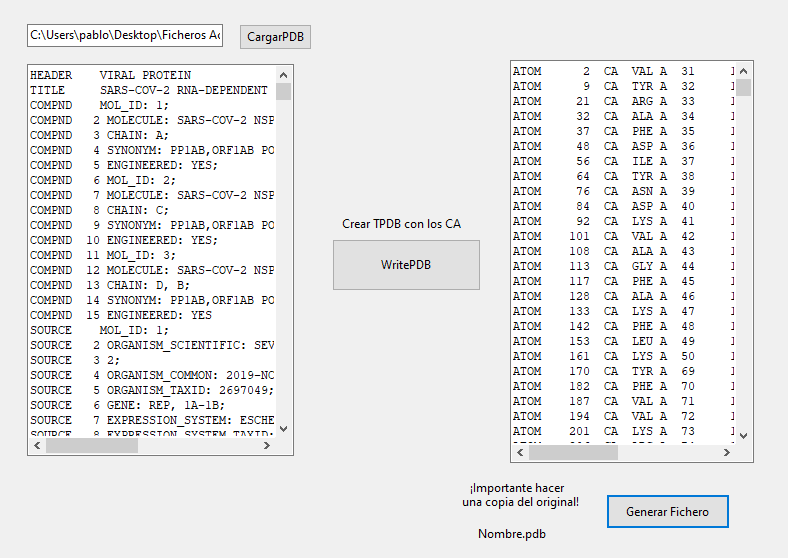
\includegraphics[width=1.1\linewidth]{Figuras/Figura12}
		\caption{Imagen del funcionamiento de la aplicación creada. A la derecha se puede observar cómo se genera el memo con todos los carbonos alfa.}		
	\end{subfigure}

	\begin{subfigure}[h]{0.45\textwidth}
		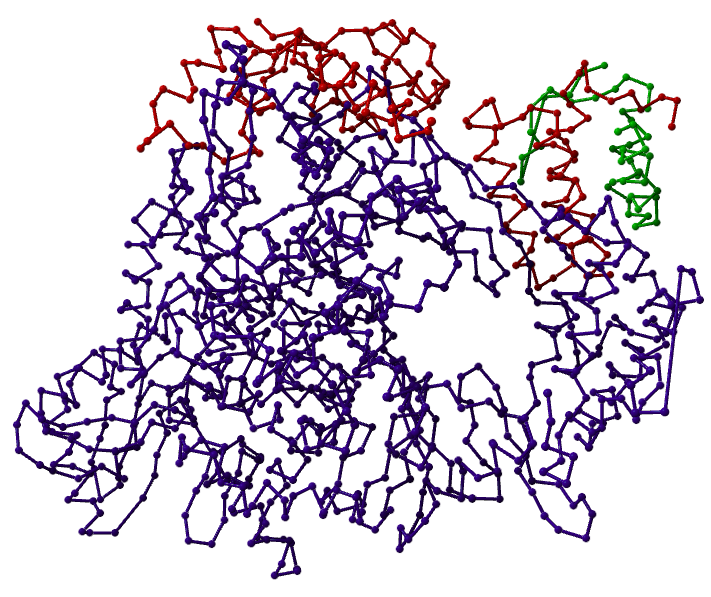
\includegraphics[width=\linewidth]{Figuras/Figura13}
		\caption{Visualización del fichero generado por writePDB, se puede observar nsp12 en negro, las dos nsp8 en rojo y nsp 7 en verde.}		
	\end{subfigure}
	\begin{subfigure}[h]{0.45\textwidth}
		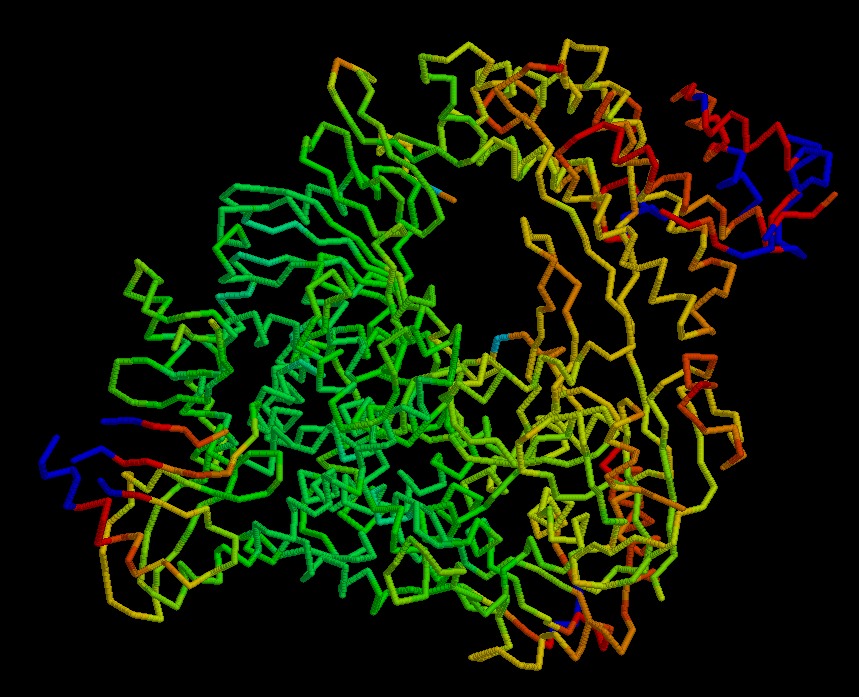
\includegraphics[width=\linewidth]{Figuras/Figura21}
		\caption{Representación del fichero generado en función de la temperatura}		
	\end{subfigure}
	
 \caption{Imagénes del funcionamiento del programa WritePDB}
 \label{fig: write}	
\end{figure}


 \section{Predicción estructural y rediseño de proteínas}
 \subsection{Diagrama de Ramachandran}
 \begin{figure}[htb!]
 	\centering
 	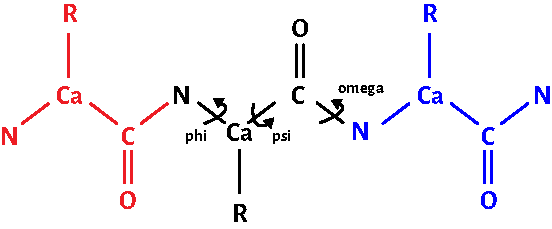
\includegraphics{Figuras/Figura14}
 	\caption{Esquema representativo del esqueleto peptídico. Los ángulos releventes van a ser $\phi$(phi) y $\psi$(psi) ya que $\omega$(omega) oscila entre valores típicos (0-180 grados). En rojo N-1, en negro el residuo N y en azul N+1}		
 \end{figure} 

 Durante el desarrollo de la asignatura se realizaron una serie de funciones capaces de calcular los distancias, ángulos de enlace y ángulos de torsión ($\phi$, $\psi$). Estos van a ser importante ya que dependiendo de cómo sea se van a poder ver patrones de estructuras secundarias características como la $\alpha$ hélice o la lámina $\beta$. Además de por esto, el diagrama de Ramachandran puede ser un indicativo de la calidad de la estructura ya que hay determinadas zonas prohibidas
 Para el cálculo de ángulos diedros:\\
 
 \begin{figure}[h]
 	\centering
 	 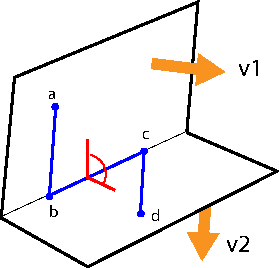
\includegraphics{Figuras/Figura46}
 	 \caption{El ángulo entre dos vectores perpendicualres es el mismo que hay entre los planos que los forman}
 \end{figure}
 
 \begin{equation}
 	\vec{v_1} \vec{v_2} = |	\vec{v_1}||\vec{v_2}|\cos\alpha
 \end{equation}
\begin{equation}
	\alpha= \arccos \frac{\vec{v_1}\vec{v_2}}{|\vec{v_1}||\vec{v_2}|}
\end{equation}
El problema es que no conocemos $\vec{v_1}$ y $\vec{v_2}$, pero lo podemos calcularas a partir de:

\begin{equation}
	\vec{v_1} = \vec{BC} \cdot \vec{BA}
\end{equation}
\begin{equation}
	\vec{v_2} = \vec{CD} \cdot \vec{CB}
\end{equation}

Para calcular estos últimos necesitamos el álgebra de vectores y calculamos los vectores de posición:
\begin{equation}
	\vec{BA} = \vec{A} - \vec{B}
\end{equation}
\begin{equation}
	\vec{BC} = \vec{C} - \vec{B}
\end{equation}
\begin{equation}
	\vec{CB} = \vec{B} - \vec{C}
\end{equation}
\begin{equation}
	\vec{CD} = \vec{D} - \vec{C}
\end{equation}
 
 Con todo esto ya podríamos hacer los cálculos necesarios para calcular el ángulo de torsión, pero es necesario primero hacer una correción de signo. Para ello se crea el vector $\vec{P}$, un vector perpendicular al plano $\vec{v_1}$, $\vec{v_2}$ ($\vec{P}$ se obtiene de realizar el producto escalar entre ambos). Este va a ser coaxial al eje y tiene dos opciones: tiene el mismo sentido que $\vec{CD}$ (giro antihorario, signo positivo) o diferente (horario, negativo). Para introducir esto en los cálculos se calcula el ángulo entre $\vec{P}$ y $\vec{CD}$ ($\gamma$) y se actualiza a lo siguiente:

 \begin{equation}
 	\alpha= \arccos \frac{\vec{v_1}\vec{v_2}}{|\vec{v_1}||\vec{v_2}|} \cos \gamma
 \end{equation}
 \begin{equation}
	\alpha= \arccos \frac{\vec{v_1}\vec{v_2}}{|\vec{v_1}||\vec{v_2}|} \frac{\vec{P}\vec{CD}}{|\vec{P}||\vec{CD}|}  
\end{equation}
Si tienen el mismo sentido $\gamma = 0º$ ($\cos0= 1$), mientras que si son opuestos $\gamma = 180º$ ($\cos180= -1$). Así aplicamos la correción de la IUPAC.

 Para todo esto se crearon una serie de funciones que se usaron aplicación capaz de construir el diagrama de Ramachandran, cosa que se va a aplicar a la proteína nsp12. Figura \ref{fig: rama}
 \\Para comprobar que la función correctamente se calcularon los ángulos de torsión de los cinco primeros residuos y se compararon con los obtenidos en un software online, MolProbity. \ref{tab: rama}
 \begin{table}[h!]
 	
 	\begin{tabular}{|c|c|c|c|c|c|c|}
 		\hline
 		Datos&TYR32A &ARG33A &ALA34A&PHE35A&ASP36A \\
 		\hline
 		Phi esperado&-126.65&-130.20&-76.58&-130.98&-107.21 \\
 		\hline
 		Phi calculado&-126.65&-130.20&-76.58&-130.98&-107.21 \\
 		\hline
 		Psi esperado&130.45&143.49&133.51&144.13&107.63 \\
 		\hline
 		Psi calculado&130.45&143.49&133.51&144.13&107.63 \\
 		\hline
 		
 	\end{tabular}
 	\caption{Comparación de los valores de ángulos de torsión de los cinco primeros residuos. Esperados son los obtenidos en MolProbity y calculado se corresponden con los obtenidos en la aplicación propia }
 	\label{tab: rama}
 \end{table}
 
Encontramos dos aplicaciones, Ramachandran y Ramachandran2. Ramachandran fue creada en clase y contiene un menú principal. Conforme se fueron actualizando los programas Ramachandran crea problemas y es por eso que decidí crear Ramachandran2, tienes las mismas funcionalidades.

 \begin{figure}[h!]
	\centering
	\begin{subfigure}{0.45\textwidth}
		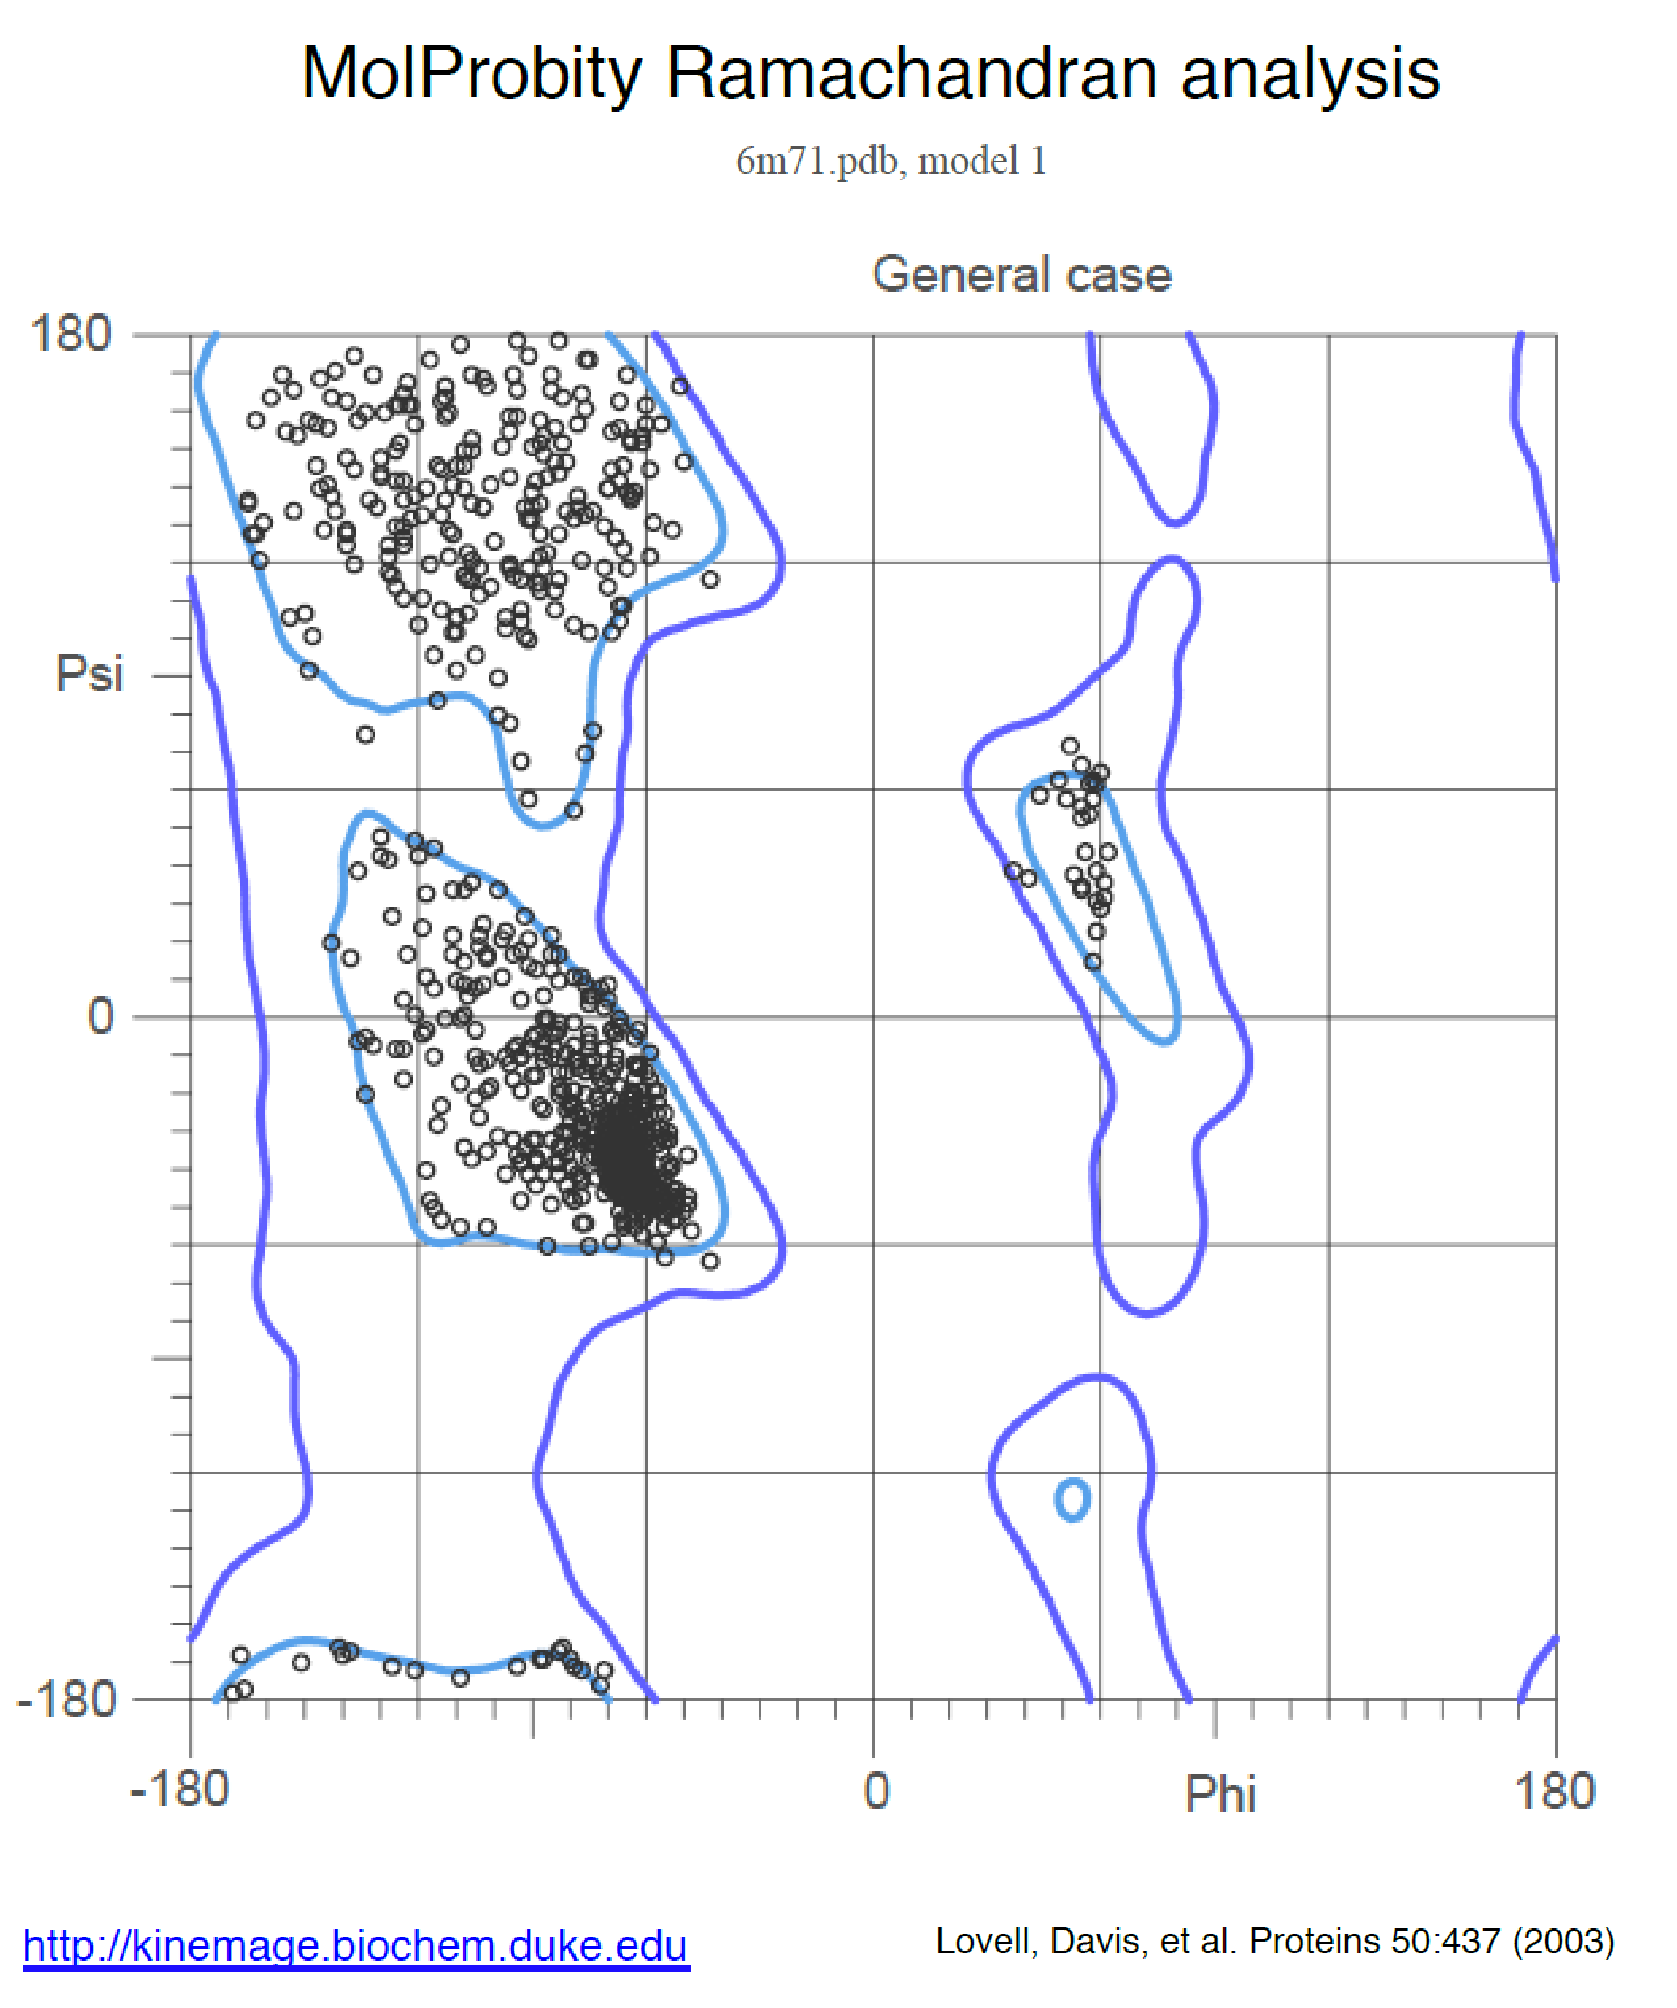
\includegraphics[width=\linewidth]{Figuras/Figura15}
		\caption{Plataforma online MolProbity }
	\end{subfigure}   
	\begin{subfigure}{0.5\textwidth}
		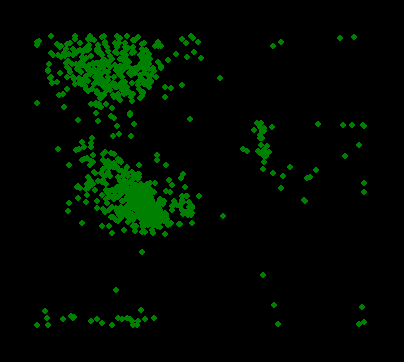
\includegraphics[width=\linewidth]{Figuras/Figura16}
		\caption{Programa propio}
	\end{subfigure}

	\begin{subfigure}{0.45\textwidth}
		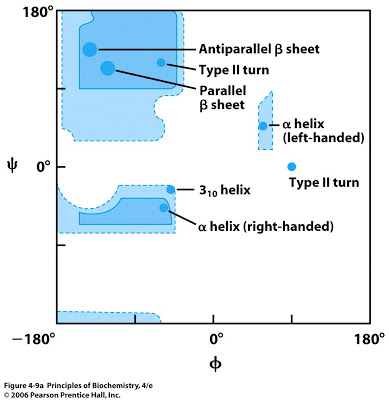
\includegraphics[width=\linewidth]{Figuras/Figura17}
		\caption{Esquema orientativo}
	\end{subfigure}

\caption{Diagramas de Ramachandran}
\label{fig: rama}	
\end{figure}



Algo interesante durante el desarrollo del programa fue la construcción de la función plotXY, que se puede ver en biotools. Esta es una herramienta muy potente que nos permite representar de manera fácil una serie de datos, pudiendo seleccionar diferentes aspectos relevantes de la representación. Además, es capaz de redimensionarse automáticamente para que la representación sea correcta.
 \subsection{Transformación de coordenadas y construcción de estereodiagrama}
 A lo largo de la asignatura se crearon una serie de funciones para poder girar o mover la estructura proteica para poder representarla o moverla según lo que nos interese.  Estas nos permite realizar transformaciones dentro del espacio afín, que se pueden ver dentro de biotools con sus respectivas explicaciones.
 Para la segunda parte se creó otra aplicación denominada Esterodiagrama. Esta carga un archivo pdb, realiza un giro de 5º sobre el eje OY y utiliza la función writePDB para generar un fichero con la estructura girada. Entonces se carga tanto el pdb original como el girado en Yasara. El estereodiagrama sería la figura \ref{estereo}.
 
  \begin{figure}[h!]
 	\centering
 	\begin{subfigure}{0.45\textwidth}
 		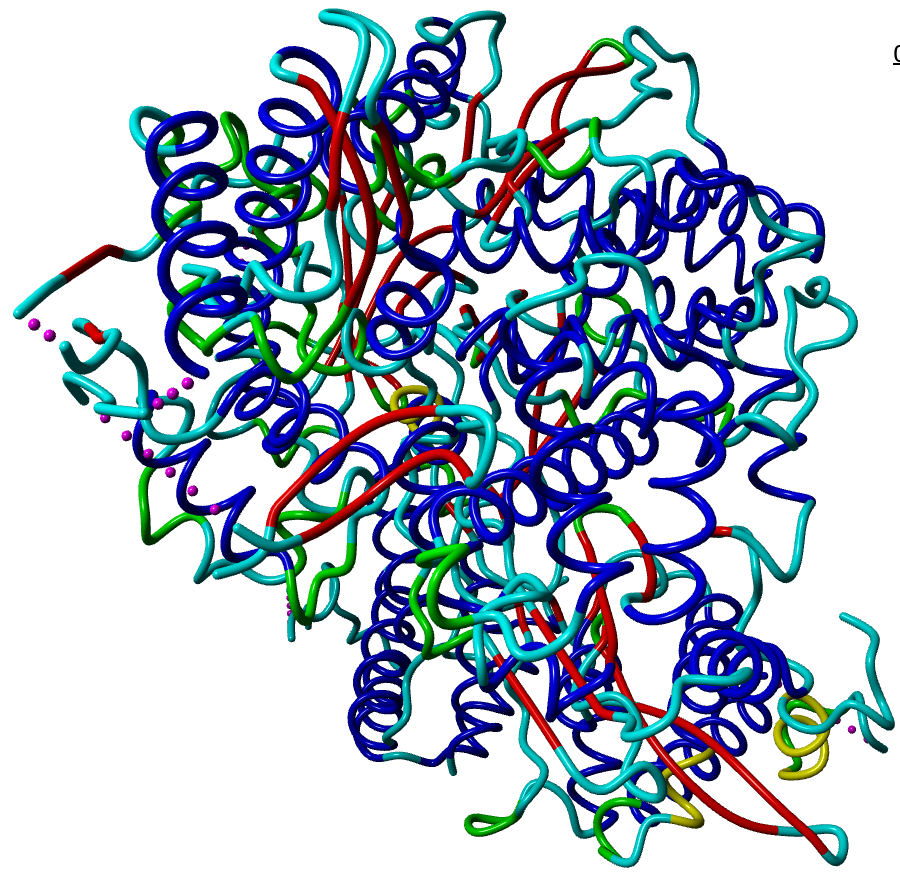
\includegraphics[width=\linewidth]{Figuras/Figura18}
 		\caption{Original }
 	\end{subfigure}   
 	\begin{subfigure}{0.45\textwidth}
 		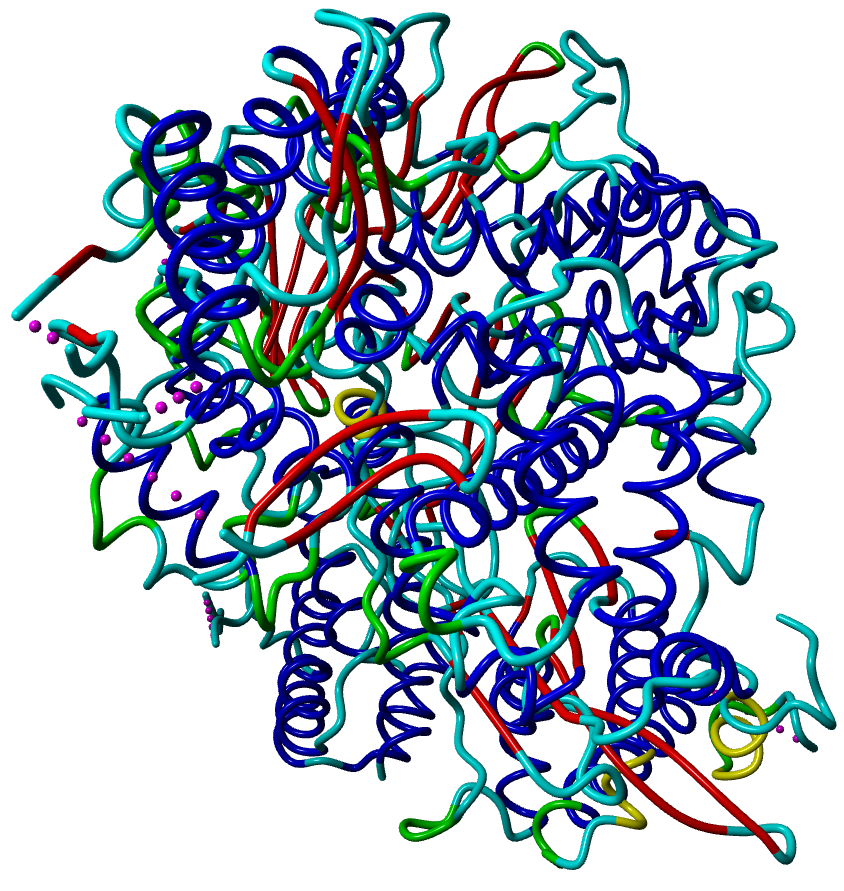
\includegraphics[width=\linewidth]{Figuras/Figura19}
 		\caption{Giro de 5º}
 	\end{subfigure}
 	
 	\caption{Estereodiagrama}
	\label{estereo}
 \end{figure}

 
 \subsection{Alineación al eje Z}
Para rotar un eje arbitrario habrá que trasladarlo el objeto a un eje (x, y o z) siendo normalmente al eje z. Una vez que está en el eje, se gira en torno a él (en torno al OZ en el caso de que se traslade al z) y volver a la situación original. Para ello necesitamos siete pasos:

\begin{enumerate}
	\item Traslación del P1 al (0, 0, 0) y todo su espacio con él
	\item Giro sobre OX hasta que P2 está en el plazo XZ
	\item Giro sobre OY hasta que P2 esté en el eje Z. El eje P1-P2 ya está en OZ
	\item Giro neto sobre OZ con el número de grados que se requiera
	\item Paso inverso a 3
	\item Paso inverso a 2
	\item Paso inverso a 1
\end{enumerate}
Los cálculos necesarios se ven en la Figura \ref{matri}. También a modo de explicación se ha realizado al figura \ref{GiroOX}, en la que ve se esquematiza cómo sería el giro OX.
 \begin{equation}
 	\sin \alpha = \frac{b (cateto opuesto)}{d1 (hipotenusa)}
 \end{equation}

 \begin{equation}
	\cos\alpha = \frac{c (cateto contiguo)}{d1 (hipotenusa)}
\end{equation}

\begin{equation}
	d1 = \sqrt{b^2 + c^2} 
\end{equation}

 \begin{figure}[h]
	\centering
	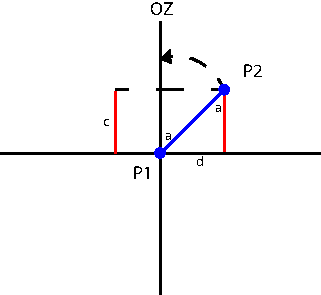
\includegraphics[width=0.5\textwidth]{Figuras/Figura36}
	\caption{Esquema del GIRO en torno a OX}
	\label{GiroOX}
\end{figure}
En este ejercicio sólo se piden los tres primeros pasos y que la representación se haga de manera que los átomos 1 y último estén superpuestos

 Para la realización de la actividad se creo una aplicación (\textbf{alinearZ}) y una función con el mismo nombre. La aplicación convierte un pdb en un TTablaDatos de dos dimensiones donde se recogen las coordenadas X e Y de los carbonos $\alpha$ que se requieran, pudiendo seleccionarse la longitud a través de dos SpinEdit.
 Se representa el primer TTablaDatos (CAI), se aplica la función alinear Z y se vuelve a representar obteniendo las imágenes de la Figura \ref{aliZ}
 
   \begin{figure}[h!]
 	\centering
 	\begin{subfigure}{0.45\textwidth}
 		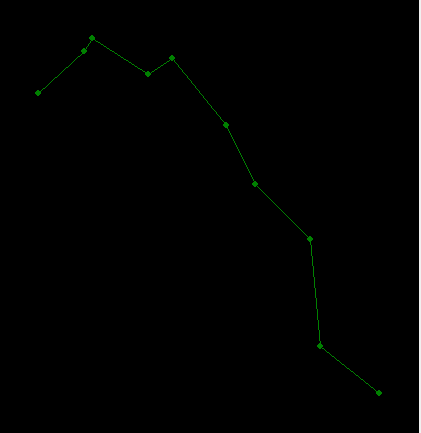
\includegraphics[width=\linewidth]{Figuras/Figura33}
 		\caption{Original}
 	\end{subfigure}   
 	\begin{subfigure}{0.45\textwidth}
 		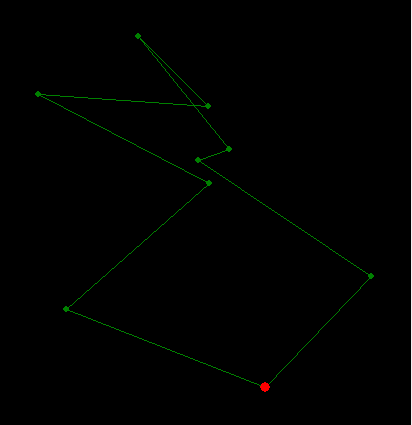
\includegraphics[width=\linewidth]{Figuras/Figura34}
 		\caption{AlinearZ aplicado}
 	\end{subfigure}
 	
 	\caption{Funcionamiento de la aplicación alinearZ}
 	\label{aliZ}
 \end{figure}
 
 Para pasar del TPDB al TTablaDatos (que es el que se puede usar en la función plotXY) se crea un tipo que sirve a modo de intermediario: TPuntos, un array de TPunto. Es importante ya éste es el tipo de dato que se requiere para el funcionamiento de las funciones realizadas.
 
 La función alinearZ se vale de otras funciones creadas, que están basadas en los pasos anteriormente explicados: traslación, GiroOX, GiroOY, GiroOZ. El paso clave es que el paso 2 es en sentido antihorario, con un ángulo $\alpha$  (positivo por convenio) y el paso 3 es horario (negativo), ángulo $\beta$. En función de en qué cuadrante nos encontremos el signo va a ser distinto para lo que se hace una corrección. Todas las explicaciones de las funciones se pueden ver en la aplicación alinearZ.
 
 \begin{figure}[h!]
 	\centering
 	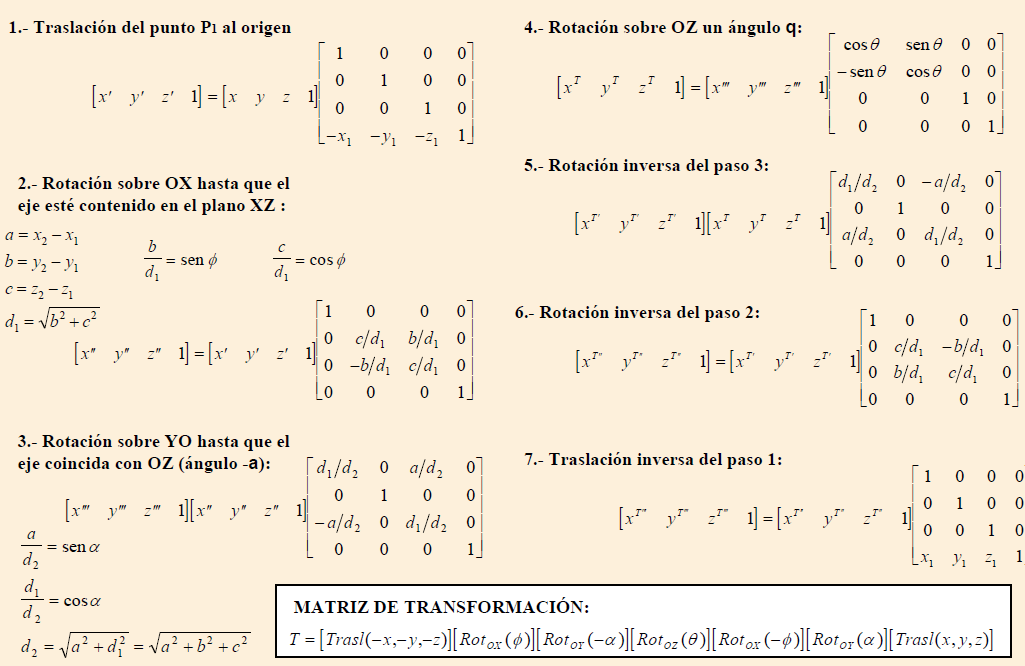
\includegraphics[width=\textwidth]{Figuras/Figura35}
 	\caption{Cálculos matriciales a realizar para la resolución. Fuente: Imágenes de la asignatura}
 	\label{matri}
 \end{figure}
 
 \subsection{Cálculo del RMSD entre las tres primeras cisteínas}
 El RMSD (Root Mean Square Desviation) o desviación cuadrática media es capaz de medirnos las diferencias entre posiciones equivalentes con el objeto de establecer cuánto se parecen o cuánto se diferencian dos determinadas características. Su aplicación a moléculas nos va a permitir establacer cómo de diferentes son dos moléculas equivalentes con diferentes formas.
 Se miden las distancias entre todos los átomos de una molécula de cisteína, para lo que creamos una tabla donde aparecen las distancias entre todos los átomos tal y como se puede ver en la figura \ref{fig: rmsd}
 \begin{figure}[h!] 
 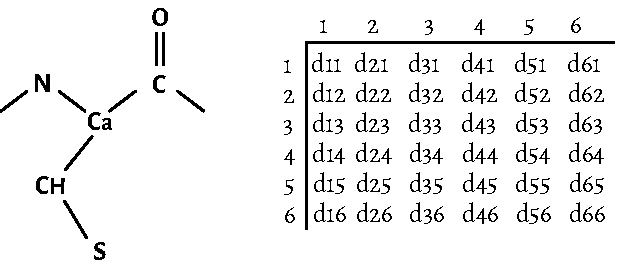
\includegraphics[width=\textwidth]{Figuras/Figura20}
 \caption{Residuo de císteina y tabla representativa de las distancias interatómicas}
 \label{fig: rmsd}
 \end{figure}

Una vez que se crea una tabla para cada una de tres primeras cisteínas se realiza el cálculo del RMSD:

\begin{equation}
	RMSD= \frac{\sqrt{\sum ((dij-dij')^2}}{n}
\end{equation}

Así comparamos las tablas de una manera que no influye cómo la cisteína esté orientada en el espacio siendo un método mucho más eficiente y fácil que otros.
Este cálculo tendría un error y esque las imágenes especulares tendrían el mismo RMSD. Sin embargo, esto no ocurre en los aminoácidos y en las proteínas por la naturaleza del enlace peptídico y de los residuos.

La aplicación se denomina RMSDapp y su funcionamiento es sencillo: en primer lugar busca las tres primeras cisteínas y una vez identificadas se pueden calcular sus RMSD. Como resultado obtenemos que las tres primeras cisteínas son los residuos 93 (1), 139 (2) y 151 (3). Sus RMSD:
\begin{table} [h]
	\centering
	\begin{tabular}{|c|c|}
		\hline
		&RMSD \\
		\hline
		Cys1-2& 2.5738\\
		Cys1-3& 2.9612\\
		Cys2-3& 1.4011\\
		\hline
	\end{tabular}
\end{table}

Cuanto más cercano a 0 sea el valor del RMSD más parecidas serán las estructuras. Al observar los residuos en cuestión de la proteína se ve que Cys93 se encuentra en un lazo, mientras que Cys139 y 151 están al inicio y final de la misma alfa hélice. Esto explicaría las diferencias observadas ya que las cisteínas 2 y 3 tienen una similitud mucho mayor entre ellas que con respecto a 1, ya que ambas están es un ambiente conformacional similar, lo que limitaría su estructura.
Por el contrario, Cys1 está en un ambiente conformacional mucho más libre.


 \subsection{Generación de mutante: Phe a Tyr}
 En esta actividad se nos pide generar una proteína mutante, cambiando una fenilalanina por una tirosina. Este cambio sólo consiste en añadir un OH a la fenilalanina ya que como se ve en el figura \ref{fig: phe} esta es la única diferencia entre los dos aminoácidos.
  \begin{figure}[h!]
 	\centering
 	\begin{subfigure}{0.45\textwidth}
 		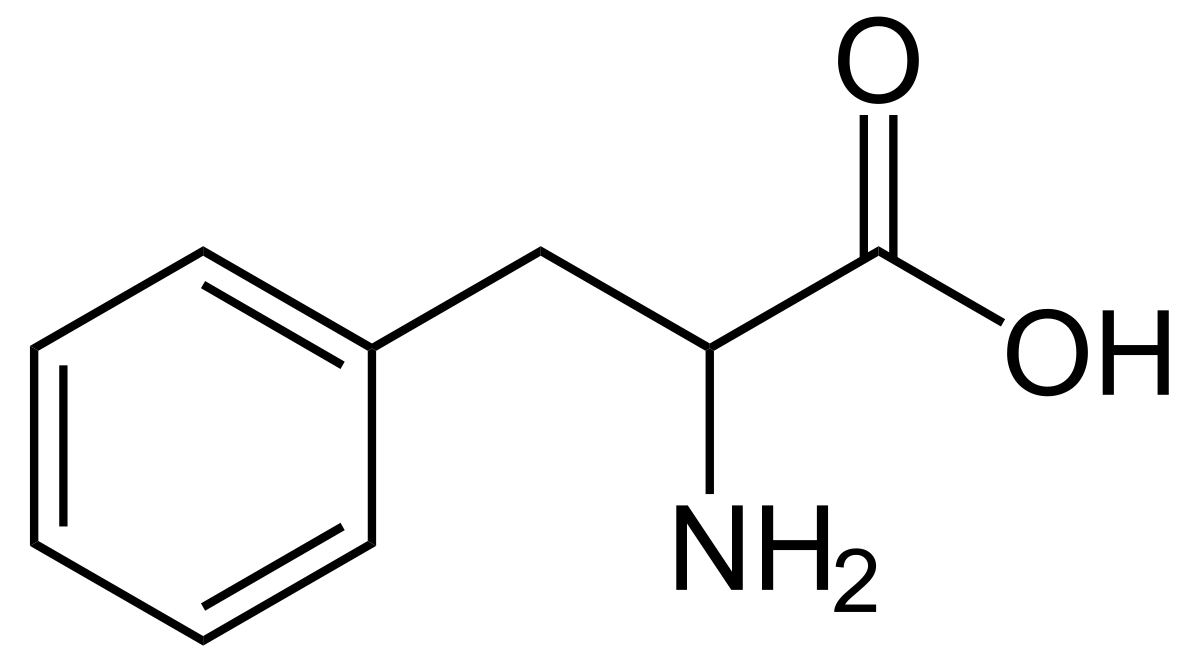
\includegraphics[width=\linewidth]{Figuras/Figura27}
 		\caption{Fenilalanina}
 	\end{subfigure}   
 	\begin{subfigure}{0.45\textwidth}
 		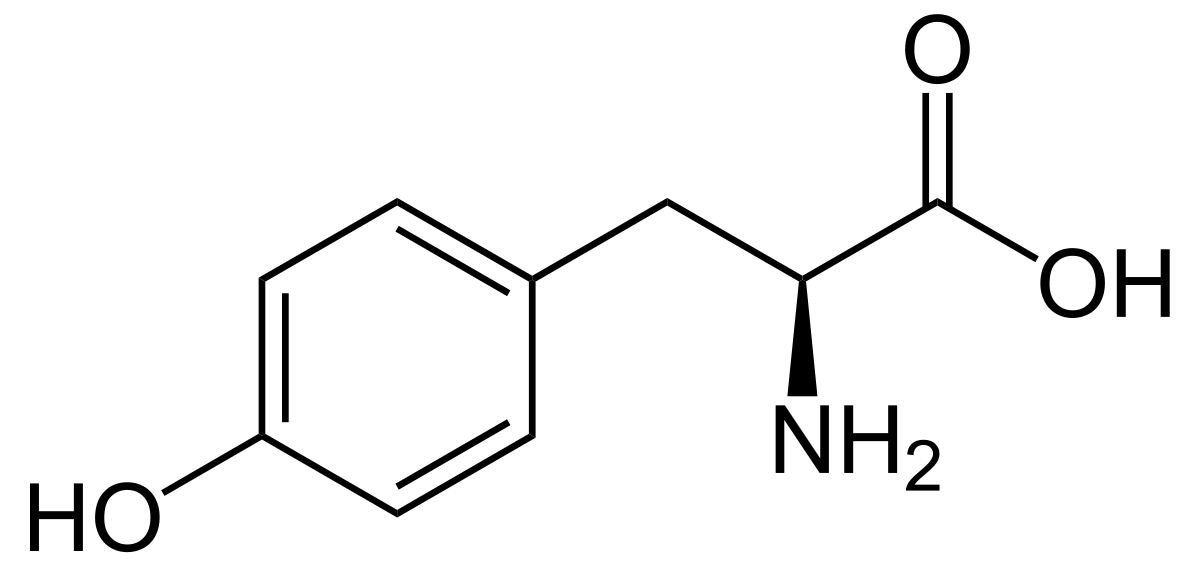
\includegraphics[width=1.1\linewidth]{Figuras/Figura28}
 		\caption{Tirosina}
 	\end{subfigure}
 	
 	\caption{Estructuras químicas de Phe y Tyr}
 	\label{fig: phe}
 	
 \end{figure}

\begin{figure}[h!]
	\centering
	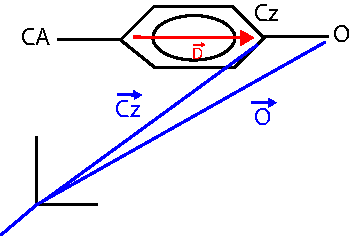
\includegraphics{Figuras/Figura29}
	\caption{Esquema de los cálculos a realizar}
	\label{fig: tyr}
\end{figure}

El problema reside en que debemos calcular cuál sería la posición del oxígeno que estamos introduciendo (el H no se tiene en cuenta). Como podemos ver en la figura \ref{fig: tyr} necesitamos calcular el vector $\vec{O}$, el cual va a ser el resultado de sumar los vectores $\vec{Cz}$ (que lo sabemos) y $\vec{v}$, siendo $\vec{v}$ el que va desde el punto Cz hasta O. $\vec{z}$ debe tener un módulo y una dirección. Para la obtención del módulo se hace una media entre las distancias entre otros tres Cz-O de otras Tyr:

\begin{equation}
	distancia = \sqrt{(X_1-X_2)^2 + (Y_1-Y_2)^2 +(Z_1-Z_2)^2}
\end{equation}
\\			
$	distancia_1 = 1.3731$ \\
$	distancia_2 = 1.3669$ 	      	\\
$	distancia_3 = 1.3700$ \\
	
$	distancia_m = 1.37 A =|\vec{v}|$

Hora sólo nos faltaría saber la dirección de de $\vec{v}$ que sería la misma que la del vector $\vec{D}$. Ésta la podemos calcular a partir de la operación $\vec{D}=	\vec{Cz}-\vec{Cb}$. Una vez tenemos esto con la ecuación \ref{eq: u} obtenemos el vector unitario $\vec{u}$, que al multiplicarlo por $|\vec{v}|$ nos dará el vector $\vec{v}$

\begin{equation}
	\frac{\vec{D}}{|\vec{D}|}= \vec{u}
	\label{eq: u}
\end{equation}

\begin{equation}
	\vec{u} \cdot |\vec{v}|= \vec{v}
	\label{eq: v}
\end{equation}

La mutación se va a hacer en la PHE287: \\
$\vec{C_Z}= (131.640, 138.287, 109.690)$ \\
$\vec{C_B}= (130.642, 141.519, 107.070)$ \\

Por tanto, $\vec{D}$ será $(0.998, -3.232, 2.614)$.

\begin{equation}
	\vec{u} = \frac{\vec{D}}{\sqrt{x^2 + y^2 + z^2}} = \frac{(0.998, -3.232, 2.614)}{4.2749} 
\end{equation}

 Así obtenemos que $\vec{u} = (0.2334, -0.7560, 0.6114)$ y podemos calcular el valor de $\vec{v}$ (Ecuación \ref{eq: v}), que sería $\vec{v}= (0.3197, -1.0357, 0.8376)$.
 
 Finalmente:
 \begin{equation}
 	\vec{O} = \vec{C_Z} + \vec{v}= (131.959, 137.251, 110.527)
 \end{equation}
Esto lo introducimos en el archivo PDB (mut01) y lo visualizamos en yasara.
 \begin{figure}[h!]
	\centering
	\begin{subfigure}{0.45\textwidth}
		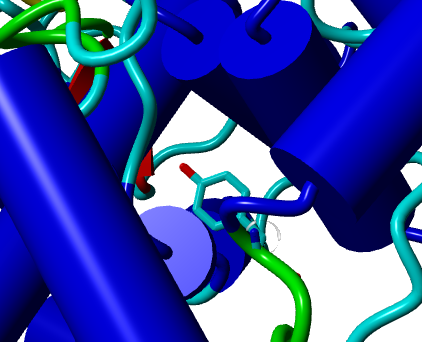
\includegraphics[width=\linewidth]{Figuras/Figura30}
		\caption{Tyr generada}
	\end{subfigure}  	
	\begin{subfigure}{0.45\textwidth}
		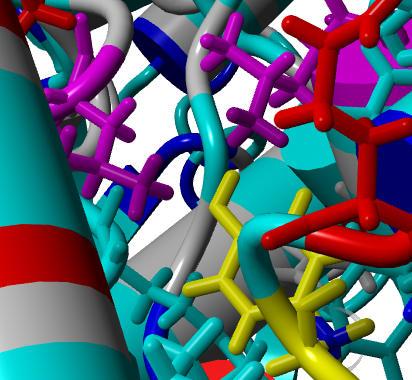
\includegraphics[width=\linewidth]{Figuras/Figura32}
		\caption{Visión del ambiente por carga. Azul: negativa, Rojo: positiva, Cyan: aa hidrofóbicos. En amarillo se puede ver la TYR y en magenta las dos leucinas}
		\label{fig: mutcar}
	\end{subfigure}
	\caption{Visualización del mutante}	
\end{figure}


El sitio donde se ha generado el mutante se corresponde con el dominio Interface de nsp12 en lo que parece ser un bolsillo hidrofóbico con una gran cantidad de anillos aromáticos. 
Como se puede observar en la figura \ref{fig: mutcar} es una zona altamente hidrofóbica. A primera vista no hay ningún tipo de impedimento estérico pero el hecho de añadir un OH a esa zona podría tener consecuencias conformacionales. Los residuos que están más cercanos en el espacio son dos leucinas (apolares) y el OH añadido seguramente disminuirá la interacción hidrofóbica que hubiese entre la Phe y las Leu como mínimo.

 \subsection{Predicción de enlaces disulfuro}
 La aplicación desarrollada se denomina enlaceSS. Su funcionamiento es sencillo, busca todos los SG (grupo tiol de las cisteínas), calcula sus distancias y si estas están por debajo de un determinado valor umbral se admite que están formando un enlace. Normalmente la distancia necesaria está entre 1-3 Amstrong por lo que se va a asumir una distancia de 3.
 Los enlaces obtenidos son:
 \begin{itemize}
 	\item CYS301A-CYS306A con una distancia de 2.71 A
 	\item CYS487A-CYS645A con una distancia de 2.16 A
 \end{itemize}

 \begin{figure}[h!]
	\centering
	\begin{subfigure}{0.45\textwidth}
		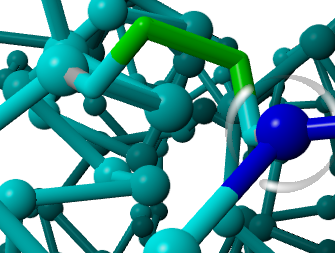
\includegraphics[width=\linewidth]{Figuras/Figura22}
		\caption{CYS301-CYS306}
	\end{subfigure}   
	\begin{subfigure}{0.45\textwidth}
		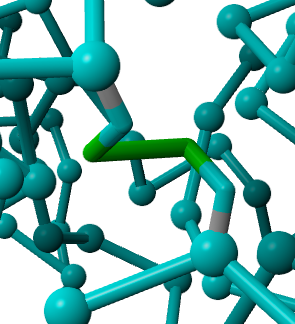
\includegraphics[width=\linewidth]{Figuras/Figura23}
		\caption{CYS487-CYS645}
	\end{subfigure}
	
	\caption{Predicción de enlaces disulfuro}
	
\end{figure}

La clave de esta asignación es dónde establecemos el umbral. Cuanto más aumentemos el umbral más sensible va a ser la predicción, pero seguramente lleve un número mayor de falsos positivos. Por el contrario, si disminuimos el umbral el porcentaje de verdaderos positivos subirá, pero los falsos negativos también.



 \subsection{Hidrofobicidad y anfipatía}
 La hidrofobicidad es un factor esencial para la estabilidad de las proteínas, siendo el factor que equilibra la balanza hacia la conformación proteica (tirón hidrofóbico). Esto es debido a que dos moléculas  hidrófobas interaccionen implica un desroden de las moléculas de agua, aumentado la entropía y disminuyendo la energía libre de Gibbs ()$\Delta G = \Delta H- T \Delta S $).
 
 Medir la hidrofobicidad de los aminoácidos (y sus residuos) es complicado. Una forma de estimación es ver cuál es la frecuencia con la que un aminoácido aparece en un bolsillo hidrofóbico. En función de como se estime, va a haber diferentes escalas de hidrofobicidad de los aminoácidos, siendo la de Doolittle una de las más importantes y la utilizada para los cálculos en este caso.
 
 Cuando se representan los \textbf{perfiles hidrofóbicos} estos tienen el problema del ruido. Para ello se realiza el suavizado de Savinsky-Golay, que consiste en calcular la hidrofobicidad media de un determinado segmento y asignársela al punto central. Poco a poco se va a aumentando el segmento hasta que se finaliza la proteína. Un detalle importante es que las ventanas generadas deben de ser impares para poder tener un residuo central.
 
 Para el programa se creó un nuevo tipo de dato, el \textbf{TTabla} siendo un array con subíndices de letras. Gracias a esta formulación podemos acceder a la hidrofobicidad de un aminoácido concreto gracias a su código de una letra. 
  
 La escala se puede cambiar en cualquier momento ya que el TEscala se genera cada vez que se quiera, permitiéndo tener una aplicación mucho más potente.  Para permitir esto se tuvo que realizar la función \textbf{CargarEscala}.
 
 Un aspecto relevante también que se extrae de la hidrofobicidad es la \textbf{anfipatía}, entendida como la distribución lateral de la hidrofobicidad en un elemento secundario. Se parte de la premisa de que las hélices serían anfipáticas, es decir, cada hemicilindro tiene una hidrofobicidad diferente. El eje de corte del hemicilindro debe variar, actualizando la anfipatía a la mayor diferencia de hidrofobicidad en cualquiera de los cortes.
 
 Para tratar de poder calcular esta anfipatía se estudiaron dos modelos: Eisenberg y Stroud.
 
 El modelo de Eisenberg está basado en el momento hidrofóbico, vectores perpendiculares a la estructura cuya magnitud hace referencia a la hidrofobicidad del residuo. Por tanto, la suma de los vectores es la hidrofobicidad total, cuya dirección y sentido indica la intensidad.
 
 \begin{equation}
 	\mu_H =\sqrt{(\sum H_n\sin(\delta n))^2+(\sum H_n \cos(\delta n))^2}
 \end{equation}
 
 $\mu_H$ es el momento hidrofóbico, el primer término se corresponde con la hidrofobicidad residual y el segundo con la distancia angular.
 
 El modelo de Stroud está basado en la parte real de la Transformada de Fourier, que permite descomponer cualquier grafo en senos y cosenos. Se representa el Power Spectrum (amplitud frente a frecuencia) a partir del cuál (en teoría) se podrá extraer información de la estructura secundaria ya que cada tipo tendrá un ritmo distinto. Por ejemplo una $\alpha$ hélice tendrá un pico en torno a 100º (no hay hélices con menos de 2 aa por vuelta) o una lámina $\beta$ tendrá picos en torno a 0 y 100º).
 
 \begin{equation}
 	I (k, v) =(\sum_{j=k-n}^{k+n} (h_j- \bar{h}(k))\sin(jv))^2 + (\sum_{j=k-n}^{k+n} (h_j- \bar{h}(k))cos(jv))^22
 \end{equation}
 
  Una vez explicado, todo estó se usó para el desarrollo de la \textbf{aplicación perfiles}, en la que se calcula tanto los perfiles hidrofóbicos como los anfipáticos (con el modelo de Stroud y Eisenberg) Aplicandolo a la proteína nsp12 (subunidad A de la estructura 6M71), los resultados obtenidos son los siguientes:
  \begin{figure}[h!]
 	\centering
 	\begin{subfigure}{\textwidth}
 		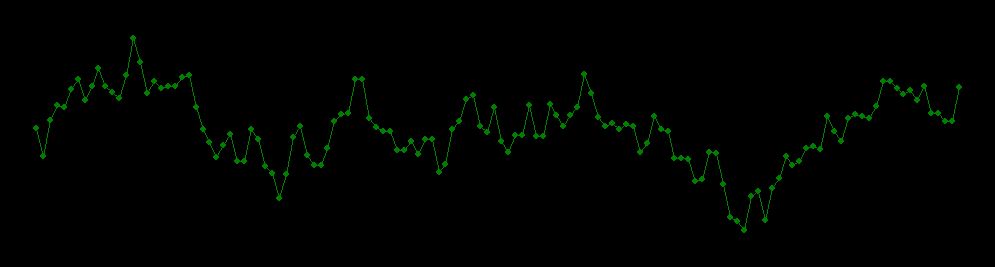
\includegraphics[width=\linewidth]{Figuras/Figura24}
 		\caption{Hidrofobicidad}
 	\end{subfigure}  
  
 	\begin{subfigure}{\textwidth}
 		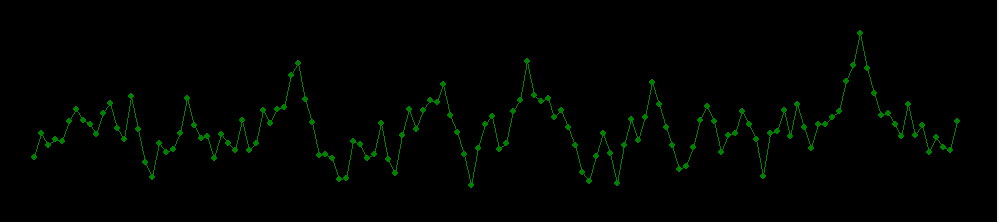
\includegraphics[width=\linewidth]{Figuras/Figura25}
 		\caption{Anfipatía según el modelo de Eisenberg}
 	\end{subfigure}
 
 	\begin{subfigure}{\textwidth}
 		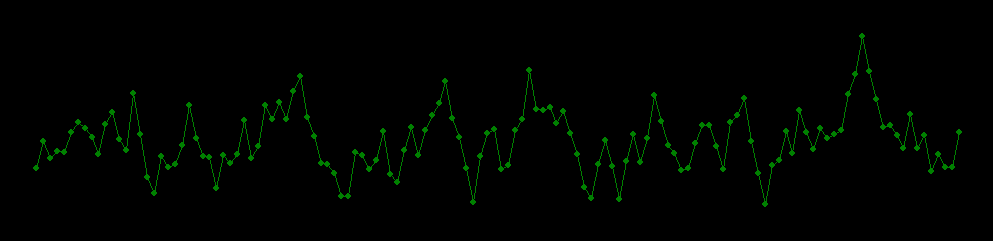
\includegraphics[width=\linewidth]{Figuras/Figura26}
 		\caption{Anfipatía según el Modelo de Stroud}
 	\end{subfigure}
 \caption{Perfiles de hidrofobicidad y anfipatía}
 \label{fig: hidrof}	
 \end{figure}

Como podemos ver en la figura \ref{fig: hidrof}, aunque se parte de conceptos distintos con ambos modelos se obtienen perfiles similares.

El código del programa se puede ver en la aplicación correspondiente (perfiles).
 
\bibliographystyle{apacite}
\bibliography{cpabib} 
\end{document}

